\documentclass[mathserif, aspectratio=169]{beamer}


\usepackage{movie15}
\usepackage{psfrag,graphicx}
\usepackage{amsmath}
\graphicspath{{figs/}}

\usetheme{Boadilla}
\makeatother
\setbeamertemplate{footline}[frame number]

\usepackage{graphicx}
\usepackage{caption}
\usepackage{subcaption}
\captionsetup{compatibility=false}
\usepackage{amsmath} 
\usepackage{amssymb} 
\usepackage{amsthm}  
\usepackage{bm}
\usepackage{lipsum}
\usepackage[linesnumbered, ruled]{algorithm2e}
\usepackage{color}
\newtheorem{assumption}{Assumptions}
\newtheorem{prop}{Proposition}
\newtheorem{defn}{Definition}
\newtheorem{thm}{Theorem}
\newtheorem{lem}{Lemma}
\newtheorem{cor}{Corollary}
\newtheorem{sol}{Decentralized Solution}
\newtheorem{thresh}{$\epsilon$-thresholding}
\definecolor{light-gray}{gray}{0.8}
\usepackage{textcomp}

\newcommand{\backupbegin}{
   \newcounter{finalframe}
   \setcounter{finalframe}{\value{framenumber}}
}
\newcommand{\backupend}{
   \setcounter{framenumber}{\value{finalframe}}
}
\newcommand{\norm}[1]{\left\lVert #1 \right\rVert}

\makeatletter
\setbeamertemplate{navigation symbols}{}


\title[Lecture 20] % (optional, use only with long paper titles)
{Data, Environment and Society: \\{Lecture 20: Model Selection and Regularization, continued}}


%\subtitle
%{Include Only If Paper Has a Subtitle}

\author[ER190C: Data, Environment and Society] 
{Instructor: Duncan Callaway\\
GSI: Seigi Karasaki} 
% - Give the names in the same order as the appear in the paper.
% - Use the \inst{?} command only if the authors have different
%   affiliation.

%\logo{
%\includegraphics[width=1.5cm,height=1.5cm,keepaspectratio]{uvic_logo_h.jpg}
%}
\vspace{-20mm}
\institute[UC Berkeley] % (optional, but mostly needed)
 {\small{ \bf October 30, 2018}}


\date[October 30, 2018]

\begin{document}

\frame{
  \titlepage
}



\begin{frame}{Recap Thursday's lecture objectives}
\begin{itemize}
\item Refine our understanding of model identification as an optimization problem
\uncover<2->{\begin{align*}
\min_\beta \sum_{i=1}^N \left(Y_i - X_i \beta \right)^2+\lambda \cdot R(\beta)\end{align*}}
\item Continue thinking about how to adjust errors to compare models with different $p$
\begin{itemize}
\item<3-> k-fold cross validation, AIC, BIC, adjusted R$^2$...
\end{itemize}
\item Understand what ``regularization'' is and why we do it
\begin{itemize}
\item<4-> A tool for adapting optimization problems to be well behaved
\item<4-> In statistical learning, a tool to tradeoff bias and variance 
\item<4-> Something that causes you to solve a different problem than the original $\rightarrow$ parameter bias
\end{itemize}
\item Understand tradeoffs between subset selection, ridge and lasso
\begin{itemize}
\item<5-> Speed (fastest to slowest): Ridge, Lasso, Subset
\item<5-> Subset selection and Lasso do feature selection.  Ridge does not.
\item<5-> You can naturally tune prediction bias-variance with Ridge and Lasso
\end{itemize}
\end{itemize}
\end{frame}

\begin{frame}{Today's objectives}

\begin{enumerate}
\item Quick review of the basic mechanics of Subset selection, Ridge and Lasso.
\item Build deeper intuition on how they work and how they differ.
\item Learn how the bias-variance tradeoff gets tuned with regularization term parameters. 
\item Understand the tradeoffs between these methods in more detail
\item Understand the importance of normalizing your variables.
\item Epilogue: the elastic net, a machine learning mashup.  
\end{enumerate}

\end{frame}

\begin{frame}{Objective 1}

Some quick review.

\end{frame}

\begin{frame}{Stepwise selection: Forward Selection}

\begin{columns}
\column{0.5\textwidth}

\textbf{Forward selection:} Start with $\mathcal{M}_0$.  Then to choose the best model from each higher ``level'':

\vspace{5mm}
\textit{First, }within each level, add one predictor at a time to the best model from the lower level.  Use $R^2$ or other to find the best model from this set of $\mathcal{M}_{k-1} \text{``}+ 1\text{''}$

\vspace{5mm}

\textit{Second,} choose from your list $\{\mathcal{M}_0, \mathcal{M}_1,...\mathcal{M}_{p}\}$ via cross validation or adjusted error metrics.\\~\\

\column{0.5\textwidth}

\vspace*{-15mm}
\begin{center}
\only<1>{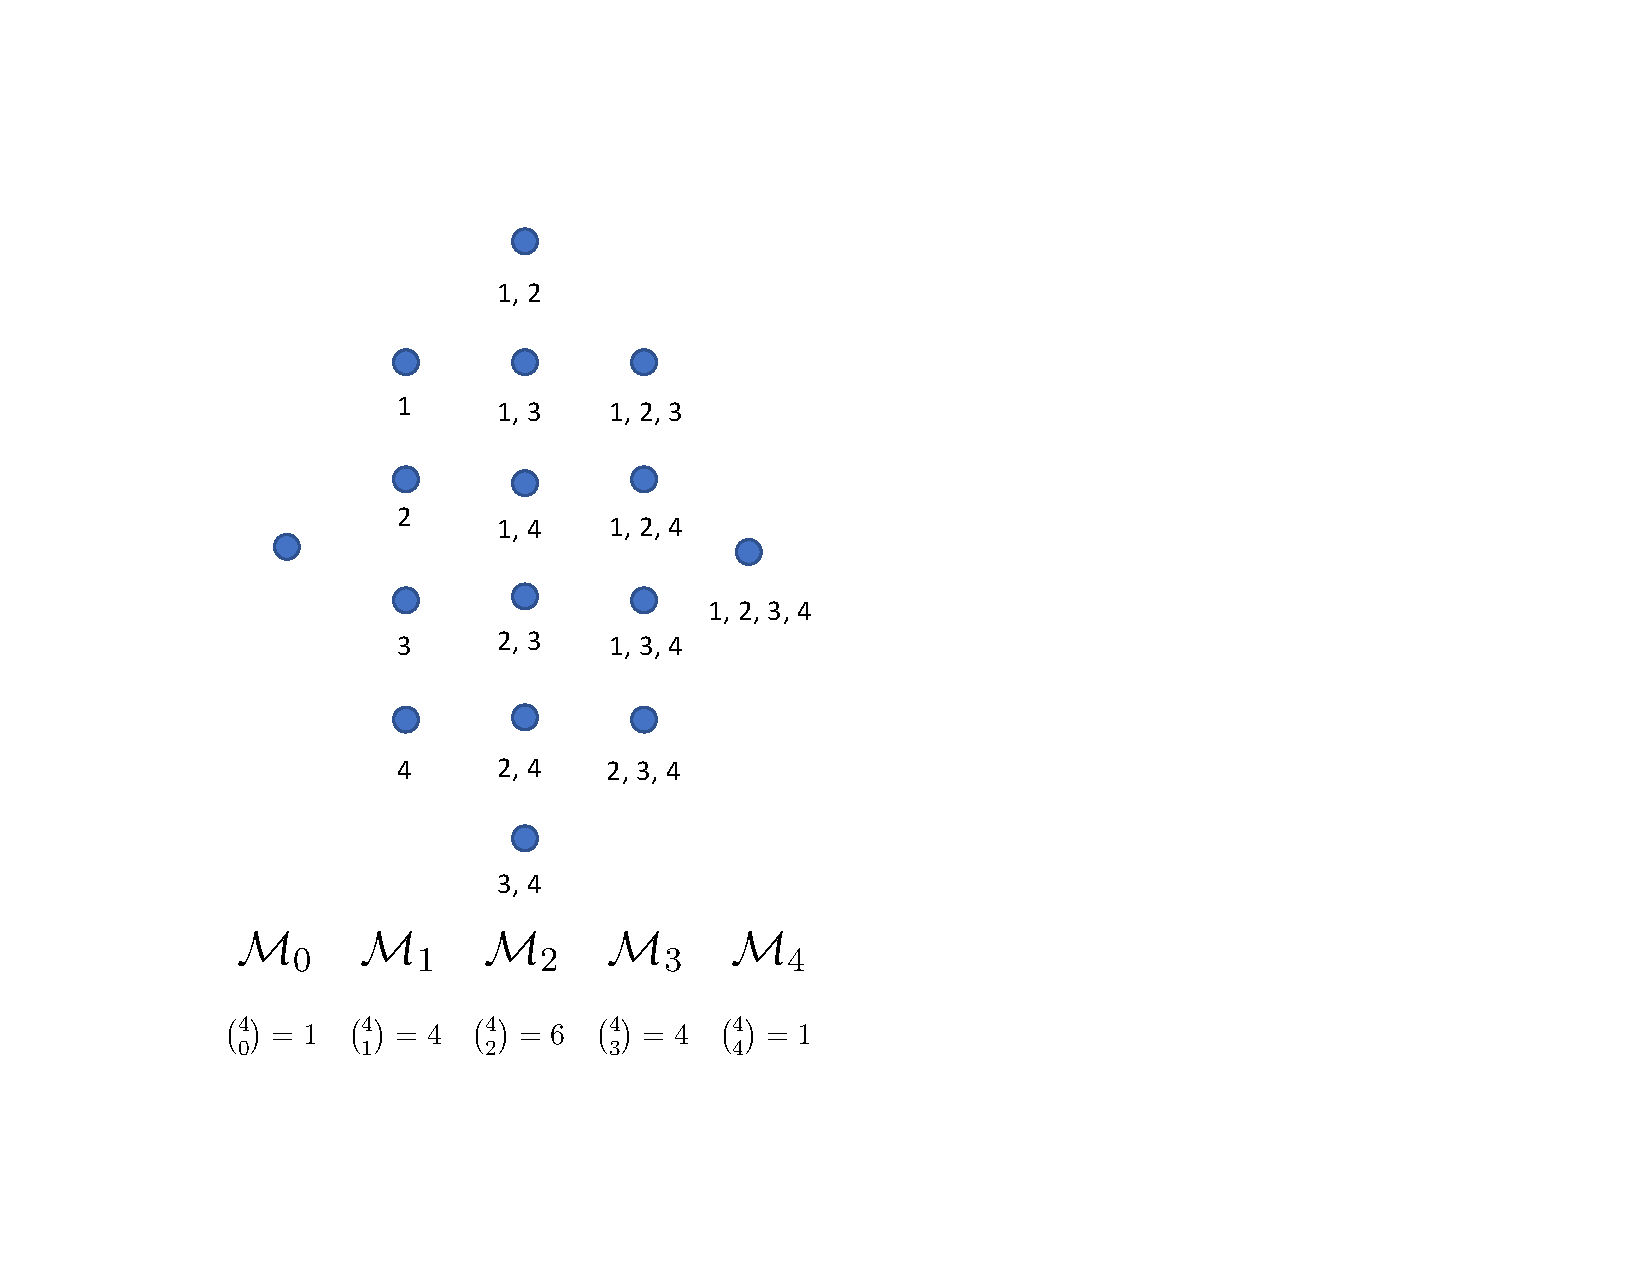
\includegraphics[scale=0.425]{4choosek}}
\only<2>{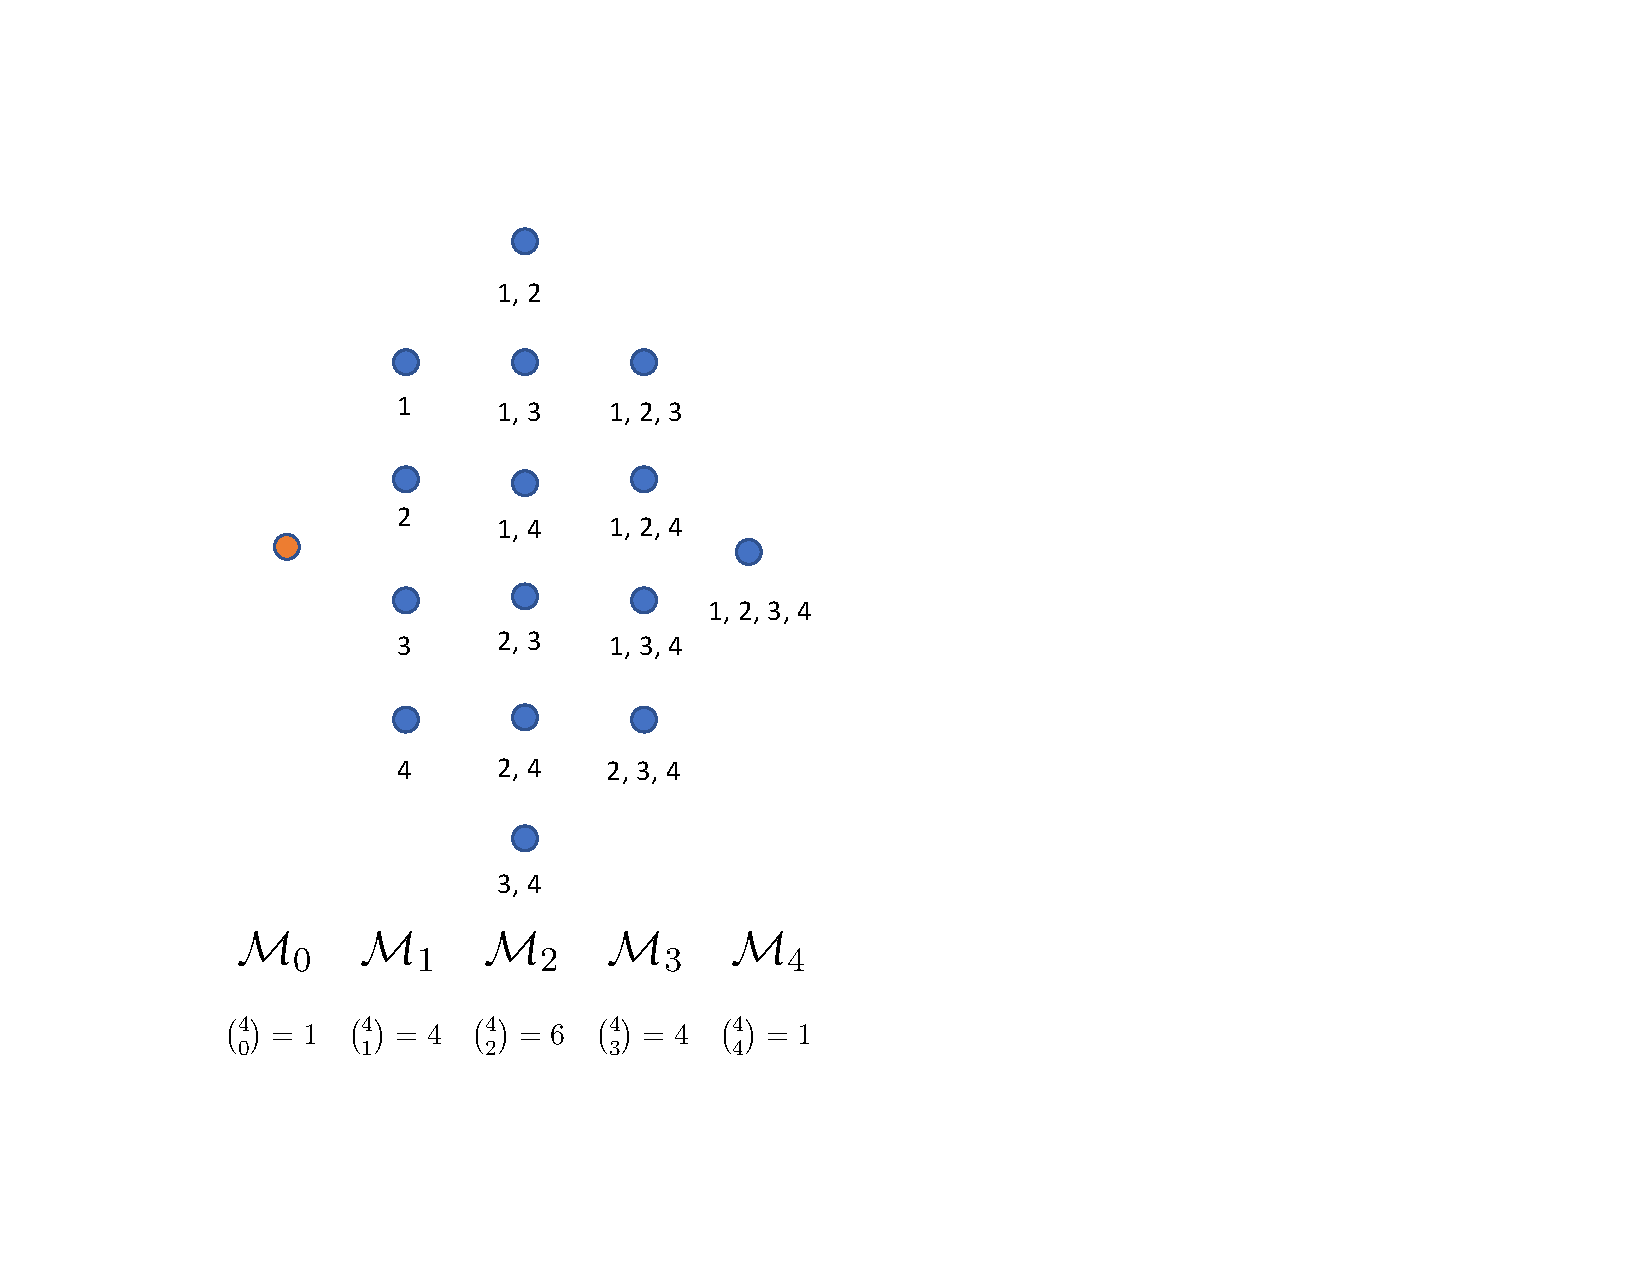
\includegraphics[scale=0.425]{4choosek_M0}}
\only<3>{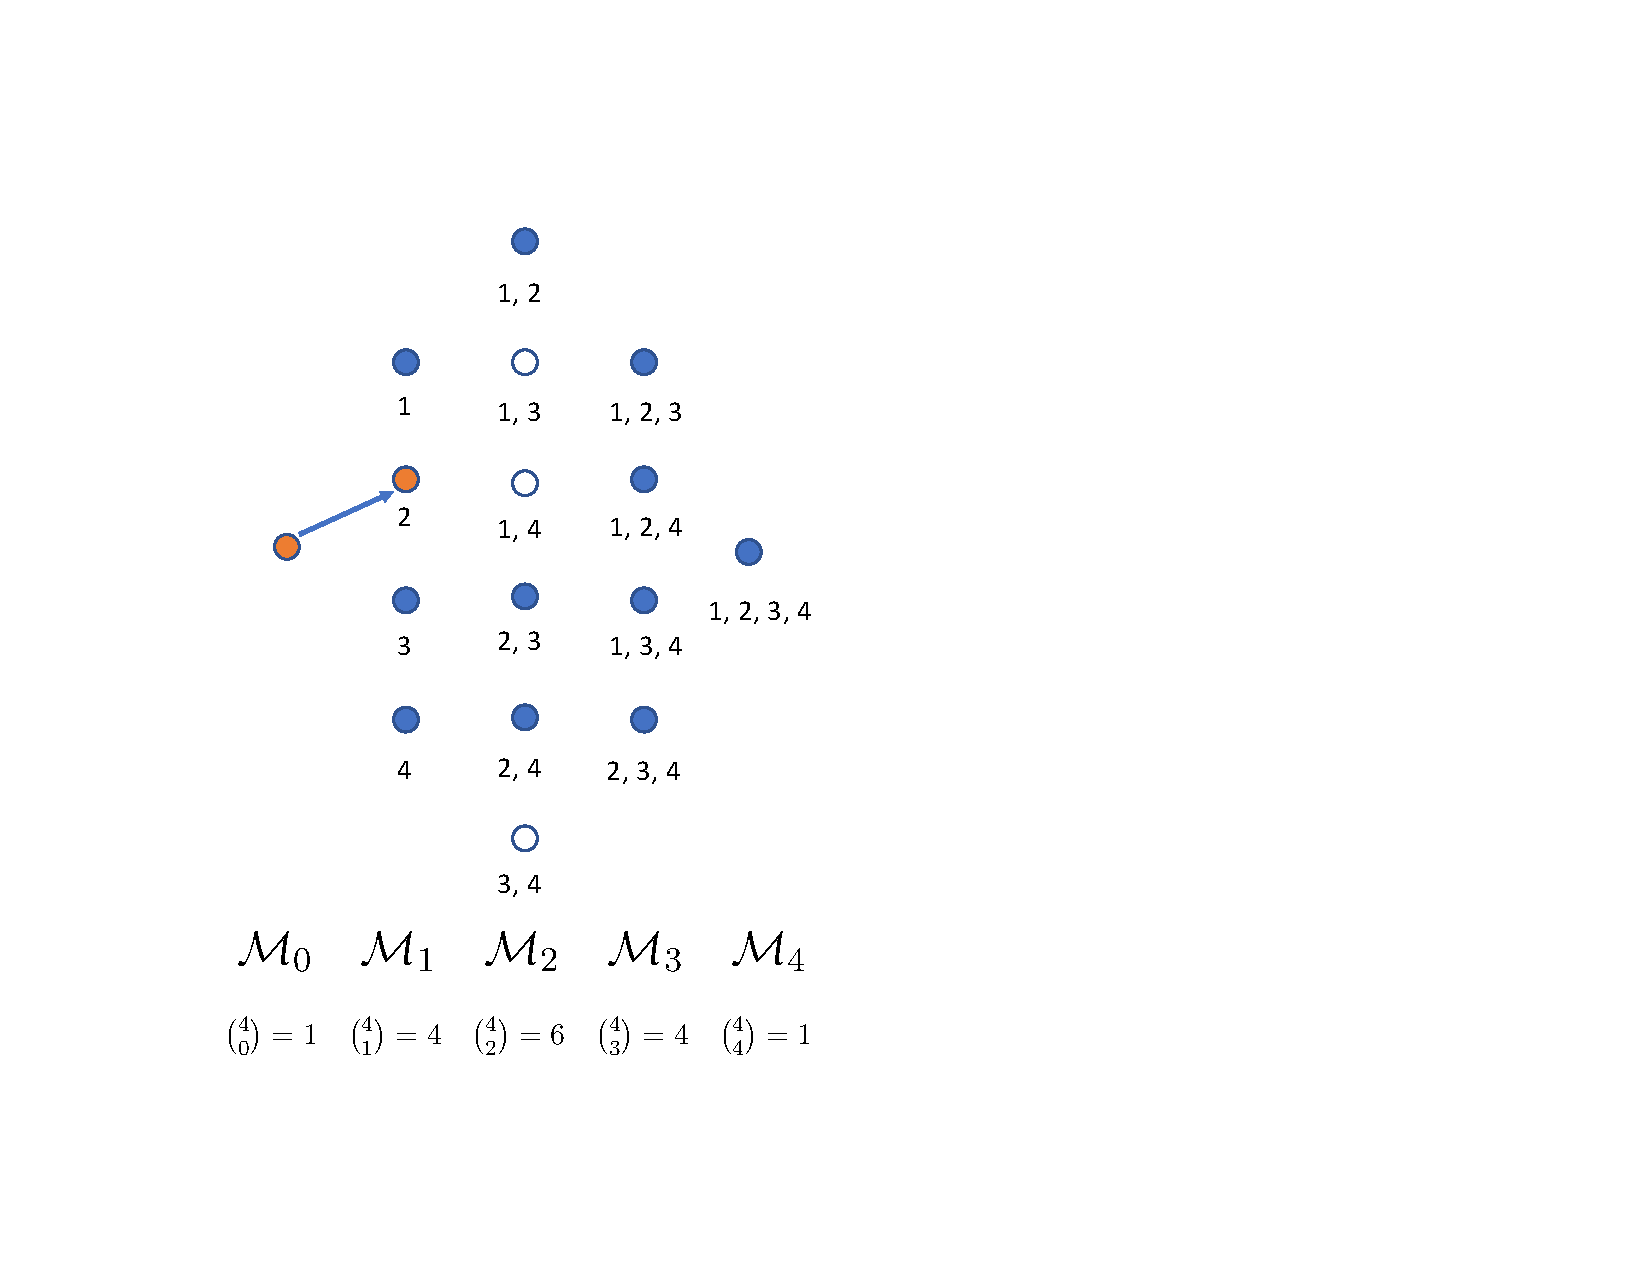
\includegraphics[scale=0.425]{4choosek_M1}}
\only<4>{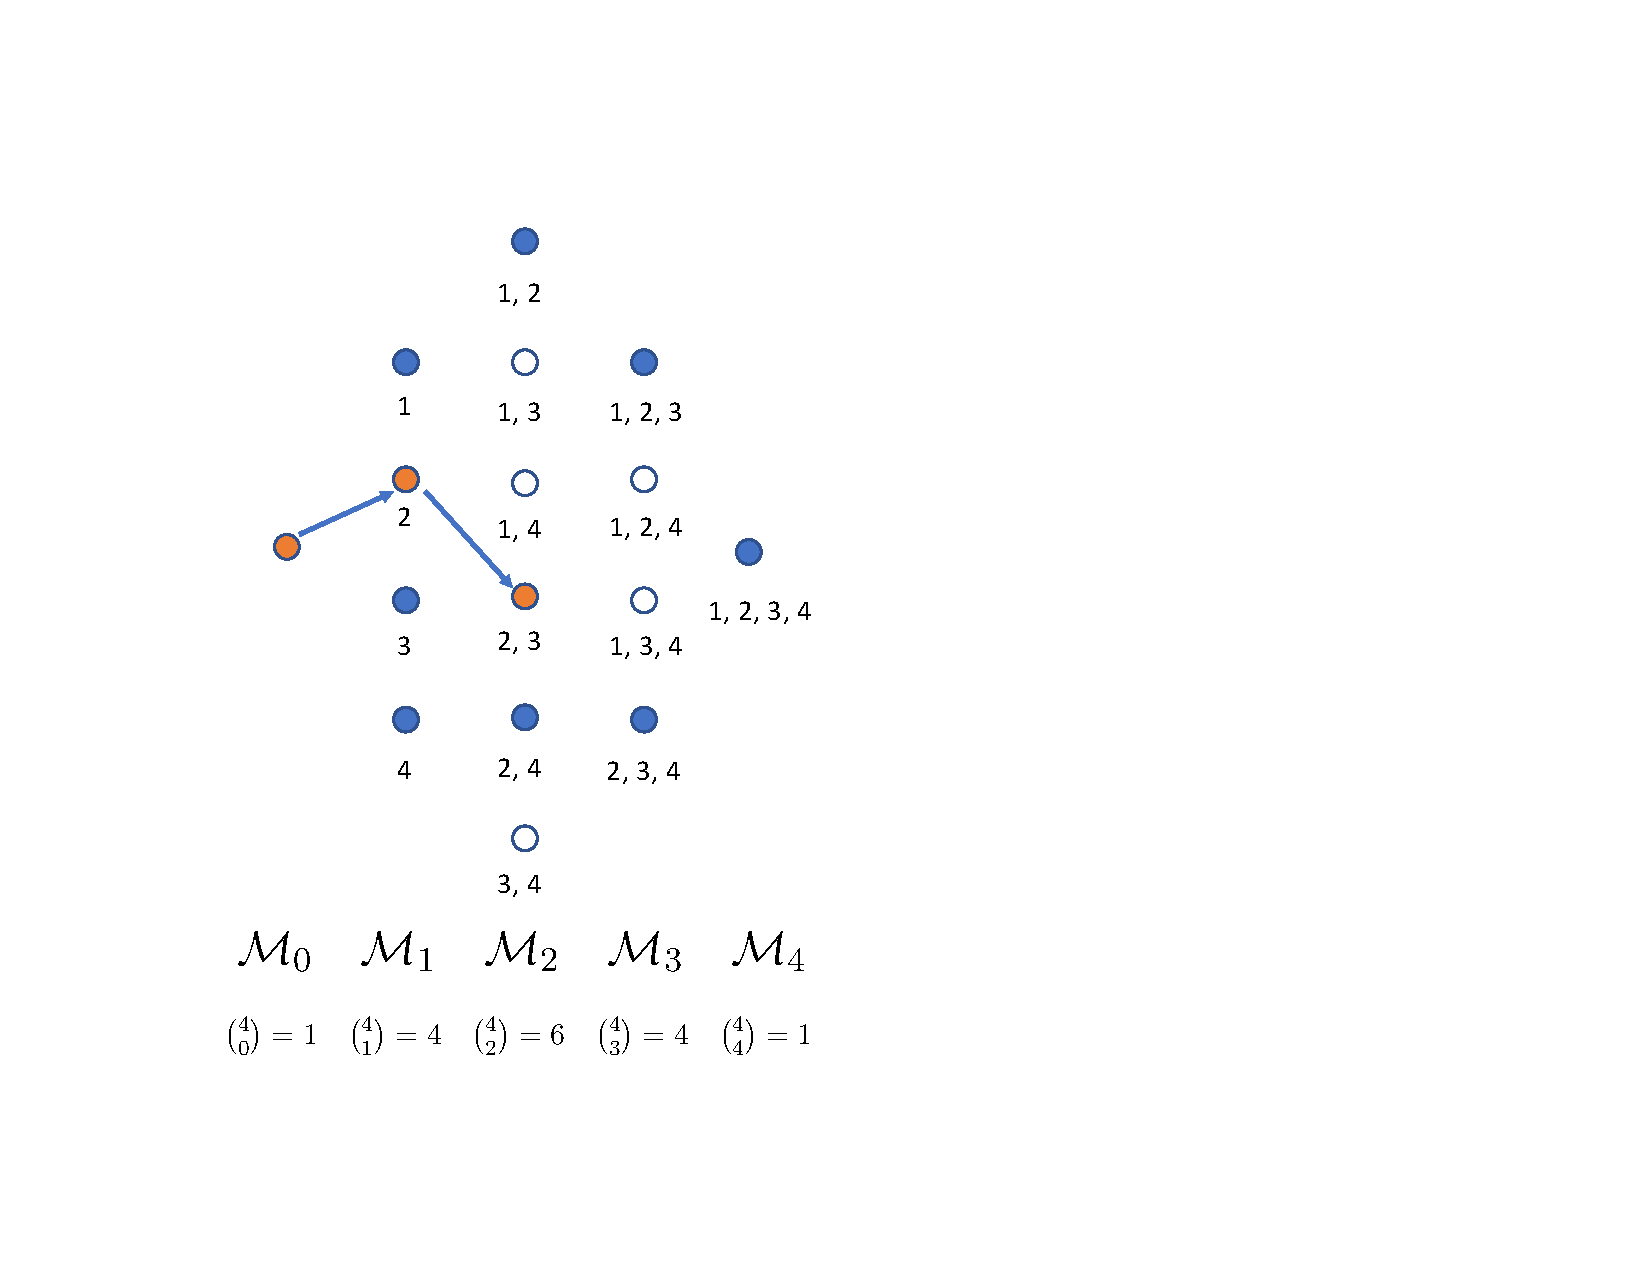
\includegraphics[scale=0.425]{4choosek_M2}}
\only<5>{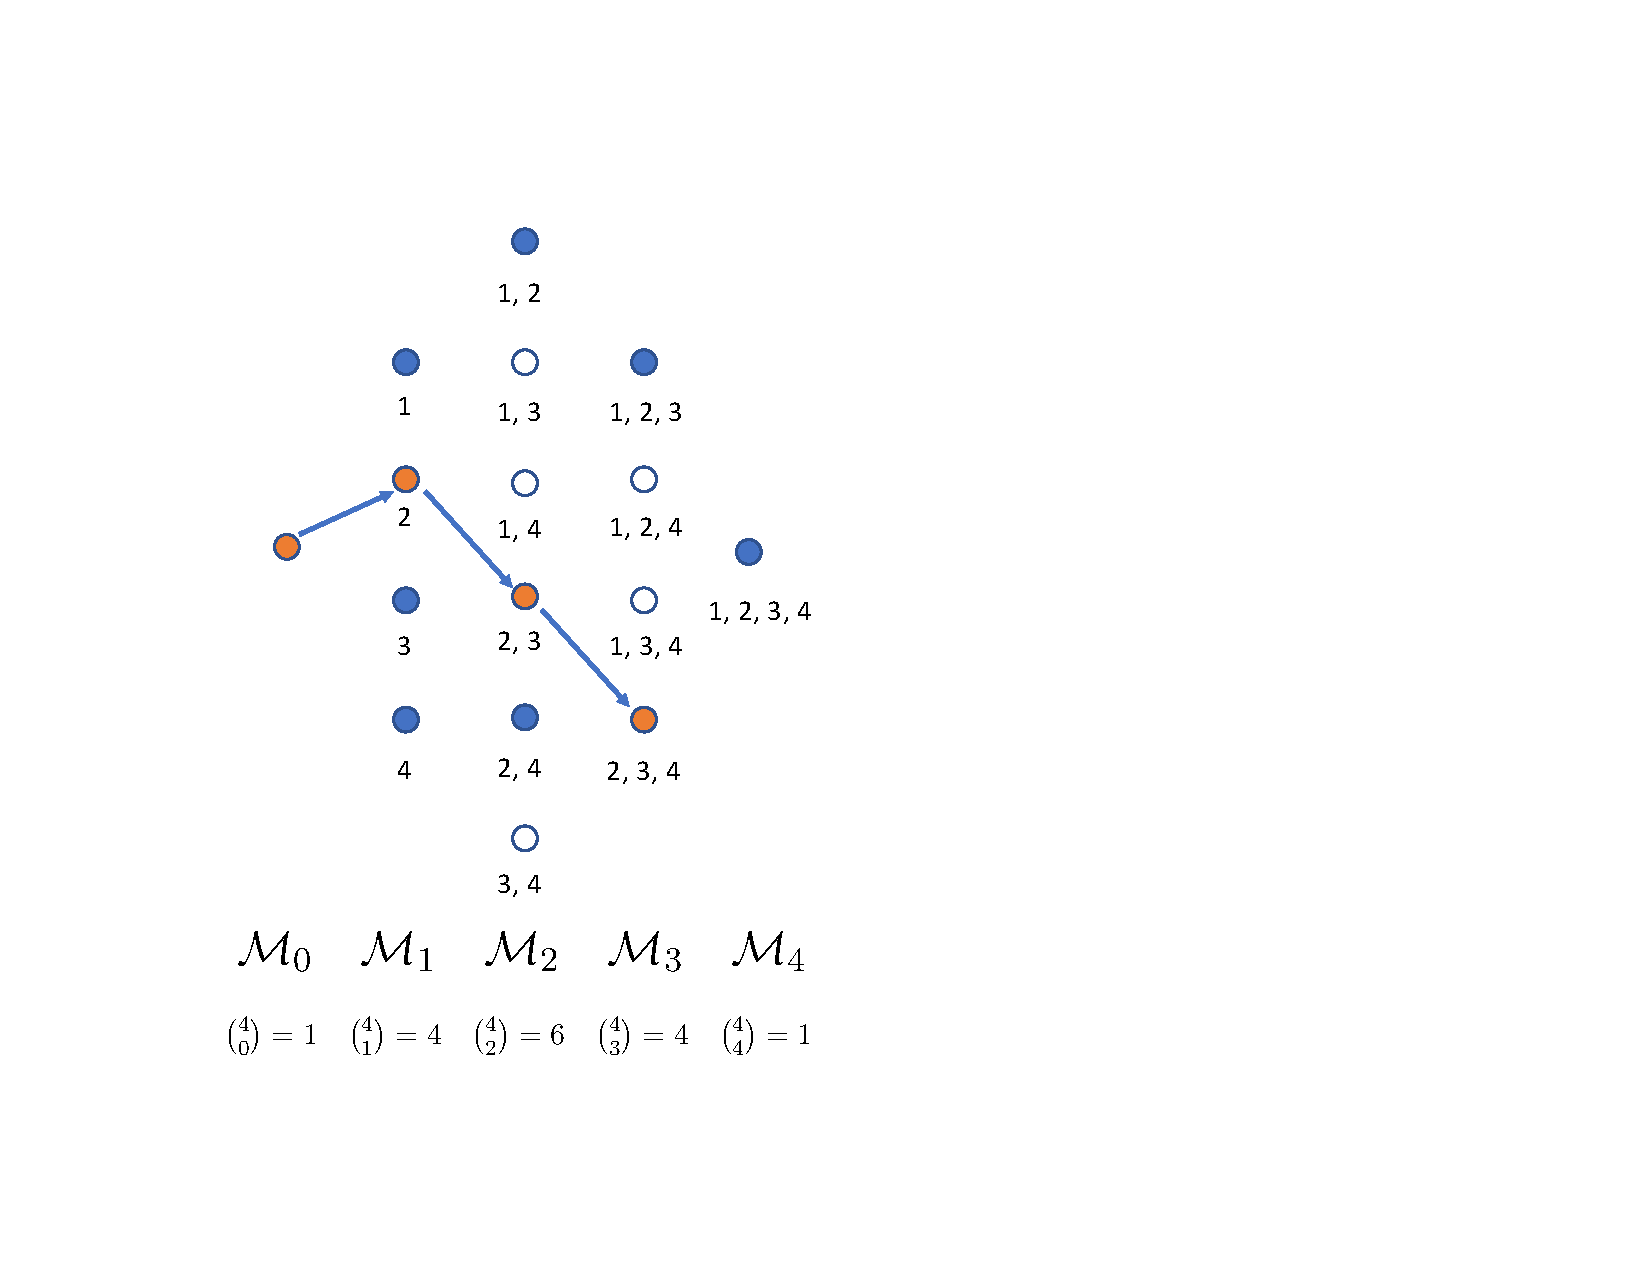
\includegraphics[scale=0.425]{4choosek_M3}}
\only<6>{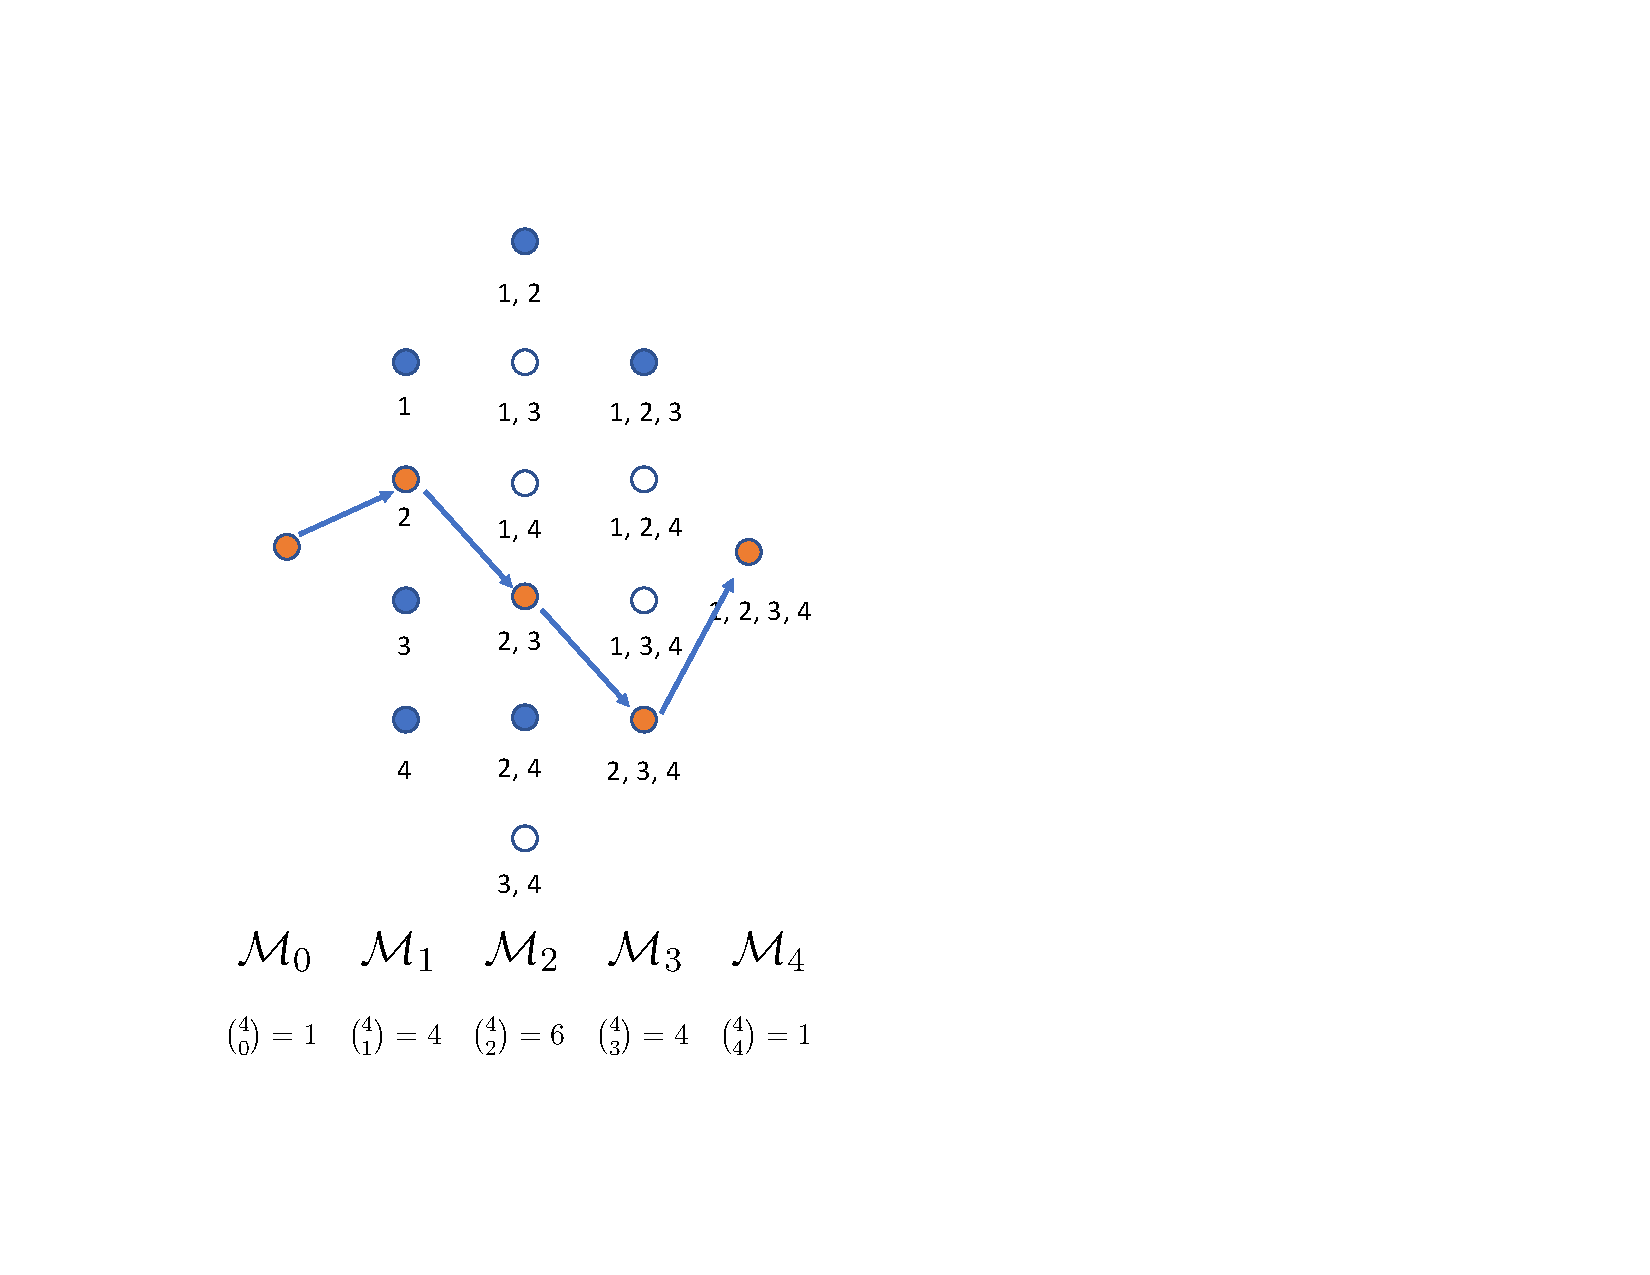
\includegraphics[scale=0.425]{4choosek_M4}}
\end{center}
\end{columns}

\end{frame}


\begin{frame}{A bit more recap}

\begin{align*}
\min_\beta \sum_{i=1}^N \left(Y_i - X_i \beta \right)^2+\lambda \cdot R(\beta)\end{align*}

The regularizing term, $R(\beta)$ can take a lot of forms.  We looked at
\begin{align*}
R(\beta) & =\sum_{i=1}^K I(\beta_i) &= \norm{\beta}_0 & \quad \text{(subset selection)} &\\
R(\beta) & =\sum_{i=1}^K |\beta_i| & = \norm{\beta}_1 & \quad \text{(lasso)} &\\
R(\beta) & =\sum_{i=1}^K \beta_i^2 & = \norm{\beta}_2^2 & \quad \text{(ridge)} &
\end{align*}

Note, last time I referred to $\sum_{i=1}^K \beta^2$ as the 2-norm.  It's not!  ($\norm{\beta}_2 = \sqrt{\sum_{k=1}^K \beta^2}$ is.)

\end{frame}


\begin{frame}{Side note:  ``Regularization''}

\textbf{Regularization} Refers to the process of adding a term to the objective function of a problem that 
\begin{itemize}
\item Makes the problem ``well behaved" (easier to solve)
\item Solves a different problem from the one you originally wanted.\\~\\
\end{itemize}

In our case, the sum of squared coefficients in Ridge makes the problem very simple to solve, but we get coefficients that are biased.\\~\\

In forecasting, the reduction in variance outweighs the growth in variance.  But what about inference? \\~\\

\pause

\begin{columns}
\column{0.6\textwidth}

Vapnik:``\textit{Regularization theory was one of the first signs of the existence of intelligent inference}''\\~\\

Why?  You avoid coefficients you shouldn't have considered.

\column{0.4\textwidth}
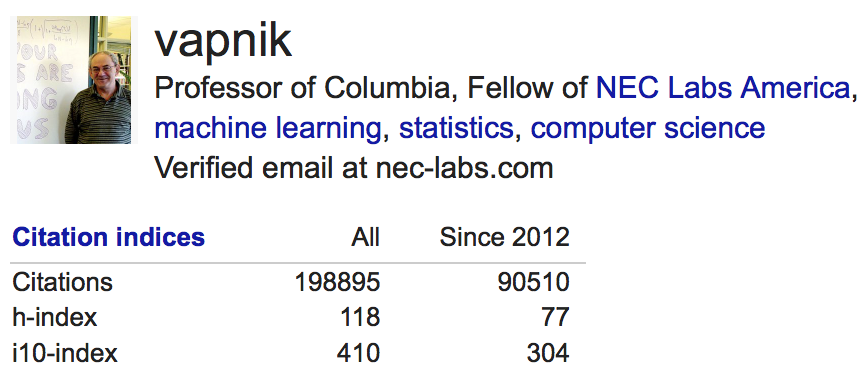
\includegraphics[scale=0.4]{vapnik}
\end{columns}
\end{frame}


\begin{frame}{Objective 2}

Building deeper intuition on how these methods work and how they differ.  
\end{frame}



\begin{frame}{Identifying parameters}

\begin{align*}
\hat{\beta}_\text{ols} = & \left(\mathbf{X}^T\mathbf{X}\right)^{-1} \left(\mathbf{X}^T\mathbf{Y}\right)\\
\hat{\beta}_\text{ridge} =& \left(\mathbf{X}^T\mathbf{X} + \lambda\mathbf{I}_k\right)^{-1} \left(\mathbf{X}^T\mathbf{Y}\right)\\
\hat{\beta}_\text{lasso}  =& \text{ Something you need to solve numerically} \\
&\text{(with something like gradient descent)}
\end{align*}

Here 
\begin{itemize}
\item $\lambda$ is a tuning parameter -- it is not unique.  
\item $\mathbf{I}_k$ is the $k\times k$ identity matrix\\~\\
\end{itemize}

\textbf{Important}! Ridge and Lasso produce different $\beta$ estimates for different choices of $\lambda$.

\end{frame}

\begin{frame}{Regularized problems can be converted to constrained problems}

\begin{align*}
\text{Subset selection:} \quad &\min_\beta \sum_{i=1}^N \left(Y_i - X_i \beta \right)^2+\lambda \cdot \sum_{k=1}^K I(\beta_k)
&\Leftrightarrow
\uncover<2->{\begin{cases}
\min_\beta \sum_{i=1}^N \left(Y_i - X_i \beta \right)^2\\
\text{subject to}\\
\sum_{k=1}^K I(\beta_k) \le s
\end{cases}}
\end{align*}

\pause
Important: 
\begin{itemize}
\item $\lambda$ and $s$ are parameters that need to be tuned. 
\item Increasing $\lambda$ has the same effect as decreasing $s$.  (Forces selection of fewer features.)
\item $\lambda$ and $s$ are not independent.  
\end{itemize}

\end{frame}


\begin{frame}{Regularized problems can be converted to constrained problems}

\begin{align*}
\text{Subset selection:} \quad &\min_\beta \sum_{i=1}^N \left(Y_i - X_i \beta \right)^2+\lambda \cdot \sum_{k=1}^K I(\beta_k)
&\Leftrightarrow
{\begin{cases}
\min_\beta \sum_{i=1}^N \left(Y_i - X_i \beta \right)^2\\
\text{subject to}\\
\sum_{k=1}^K I(\beta_k) \le s
\end{cases}}\\\\
%
\text{Ridge:} \quad  &\min_\beta \sum_{i=1}^N \left(Y_i - X_i \beta \right)^2+\lambda \cdot \sum_{k=1}^K |\beta_k|
&\Leftrightarrow
\uncover<2->{\begin{cases}
\min_\beta \sum_{i=1}^N \left(Y_i - X_i \beta \right)^2\\
\text{subject to}\\
\sum_{k=1}^K |\beta_k | \le s
\end{cases}}\\\\
%
\text{Lasso:} \quad  &\min_\beta \sum_{i=1}^N \left(Y_i - X_i \beta \right)^2+\lambda \cdot \sum_{k=1}^K \beta_k^2 
&\Leftrightarrow
\uncover<3->{\begin{cases}
\min_\beta \sum_{i=1}^N \left(Y_i - X_i \beta \right)^2\\
\text{subject to}\\
\sum_{k=1}^K \beta_k^2 \le s
\end{cases}}
\end{align*}

\end{frame}

\begin{frame}{Setting intuition about constrained problems}

Imagine a simple two-feature problem.  

\begin{columns}

\column{0.25\textwidth}
\begin{center}
No constraints.  Red lines are ``constant RSS'' contours
\end{center}
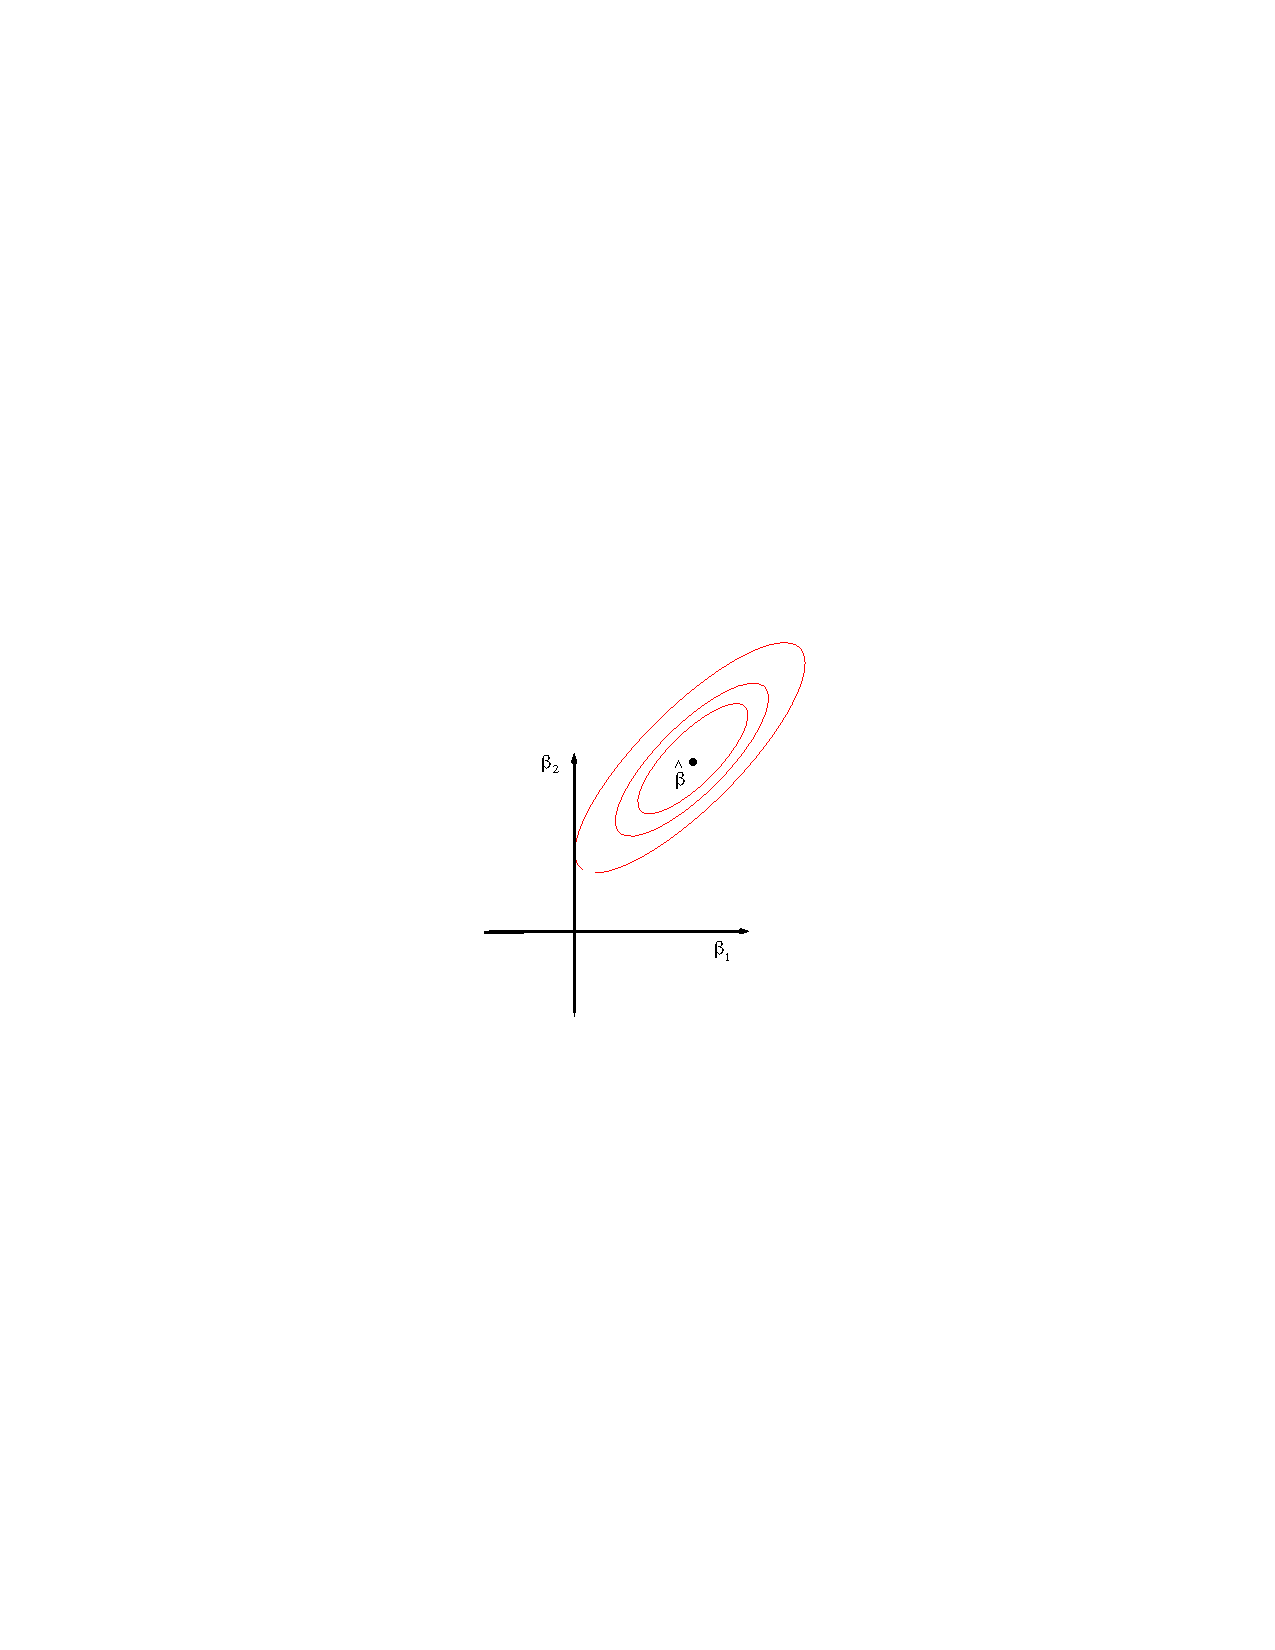
\includegraphics[scale=0.65]{RSE_contour}

\pause
\column{0.25\textwidth}
\begin{center}
Subset selection.  If $\sum_{k=1}^K I(\beta_k) \le 1$, solutions on blue lines.
\end{center}
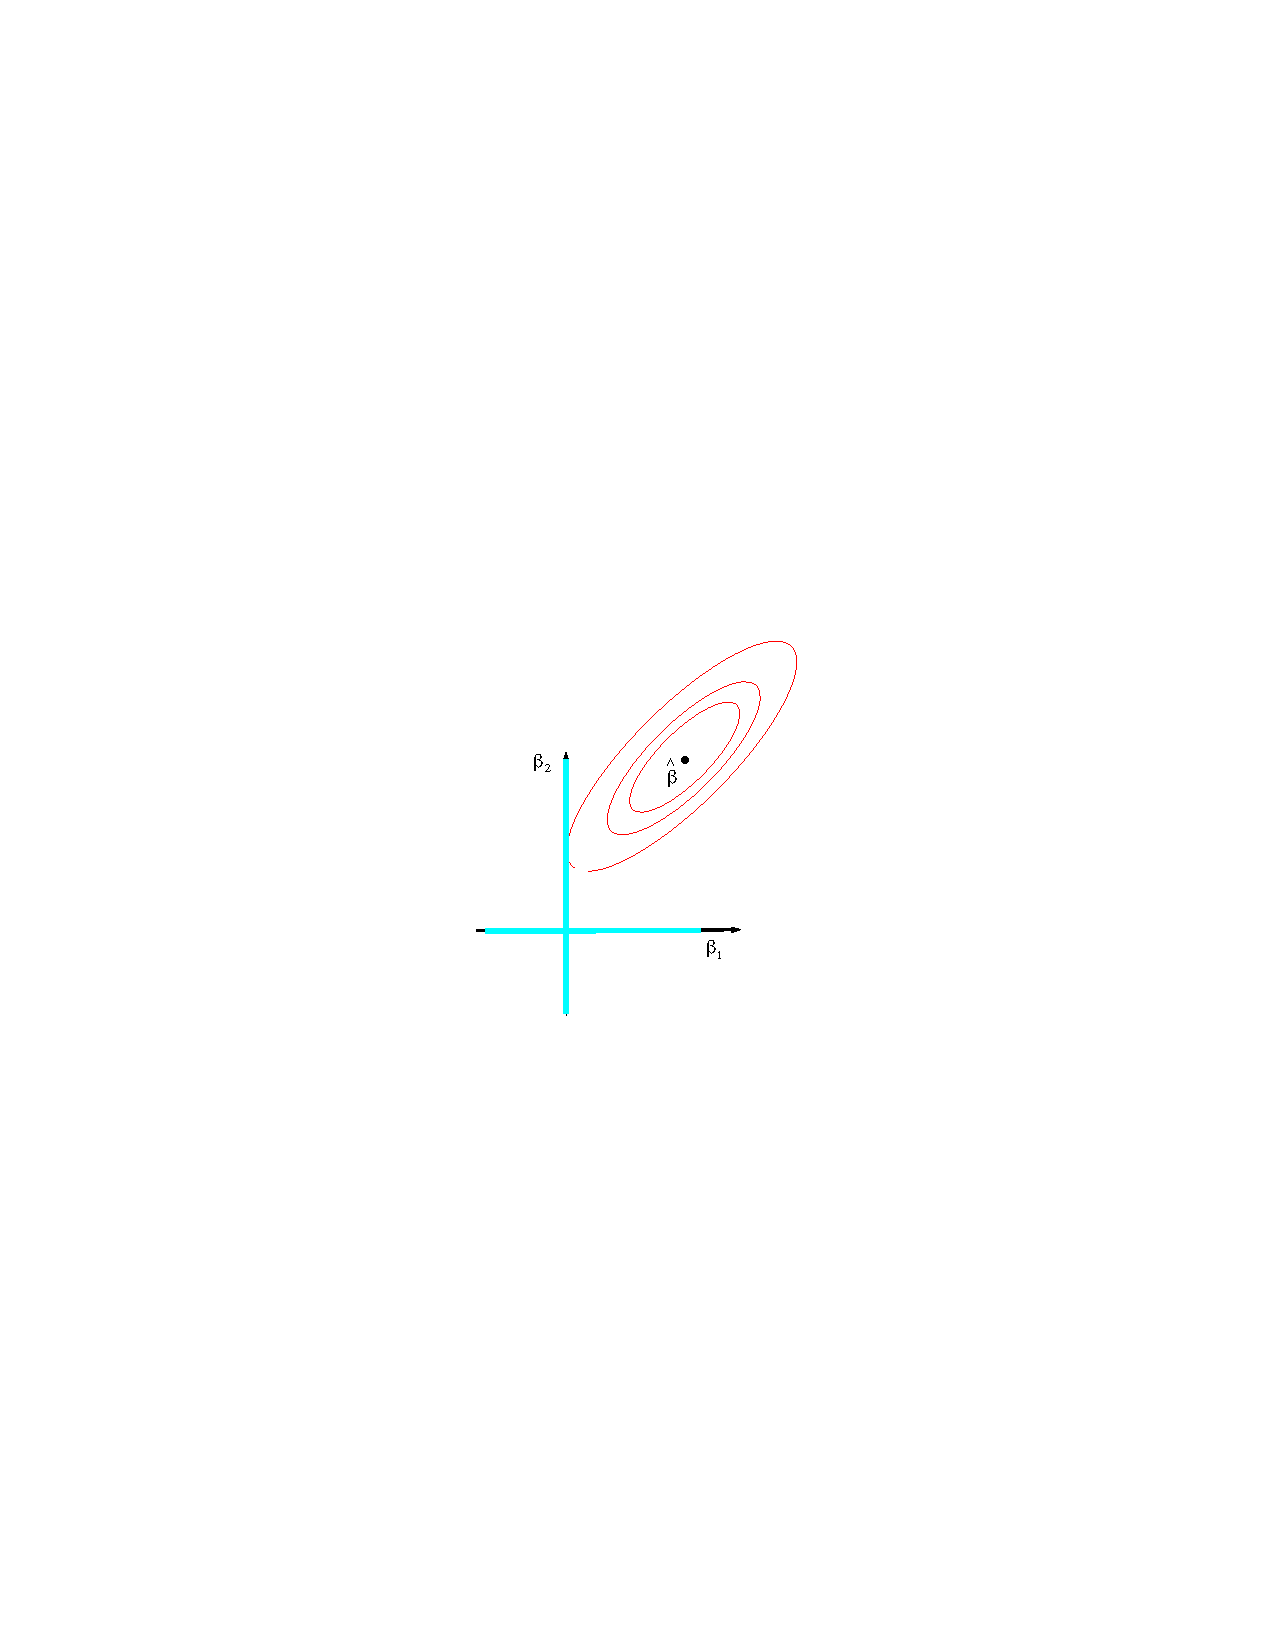
\includegraphics[scale=0.65]{RSE_subset_constr}

\pause
\column{0.25\textwidth}
\begin{center}
Lasso.   Solutions must be in blue diamond.
\end{center}
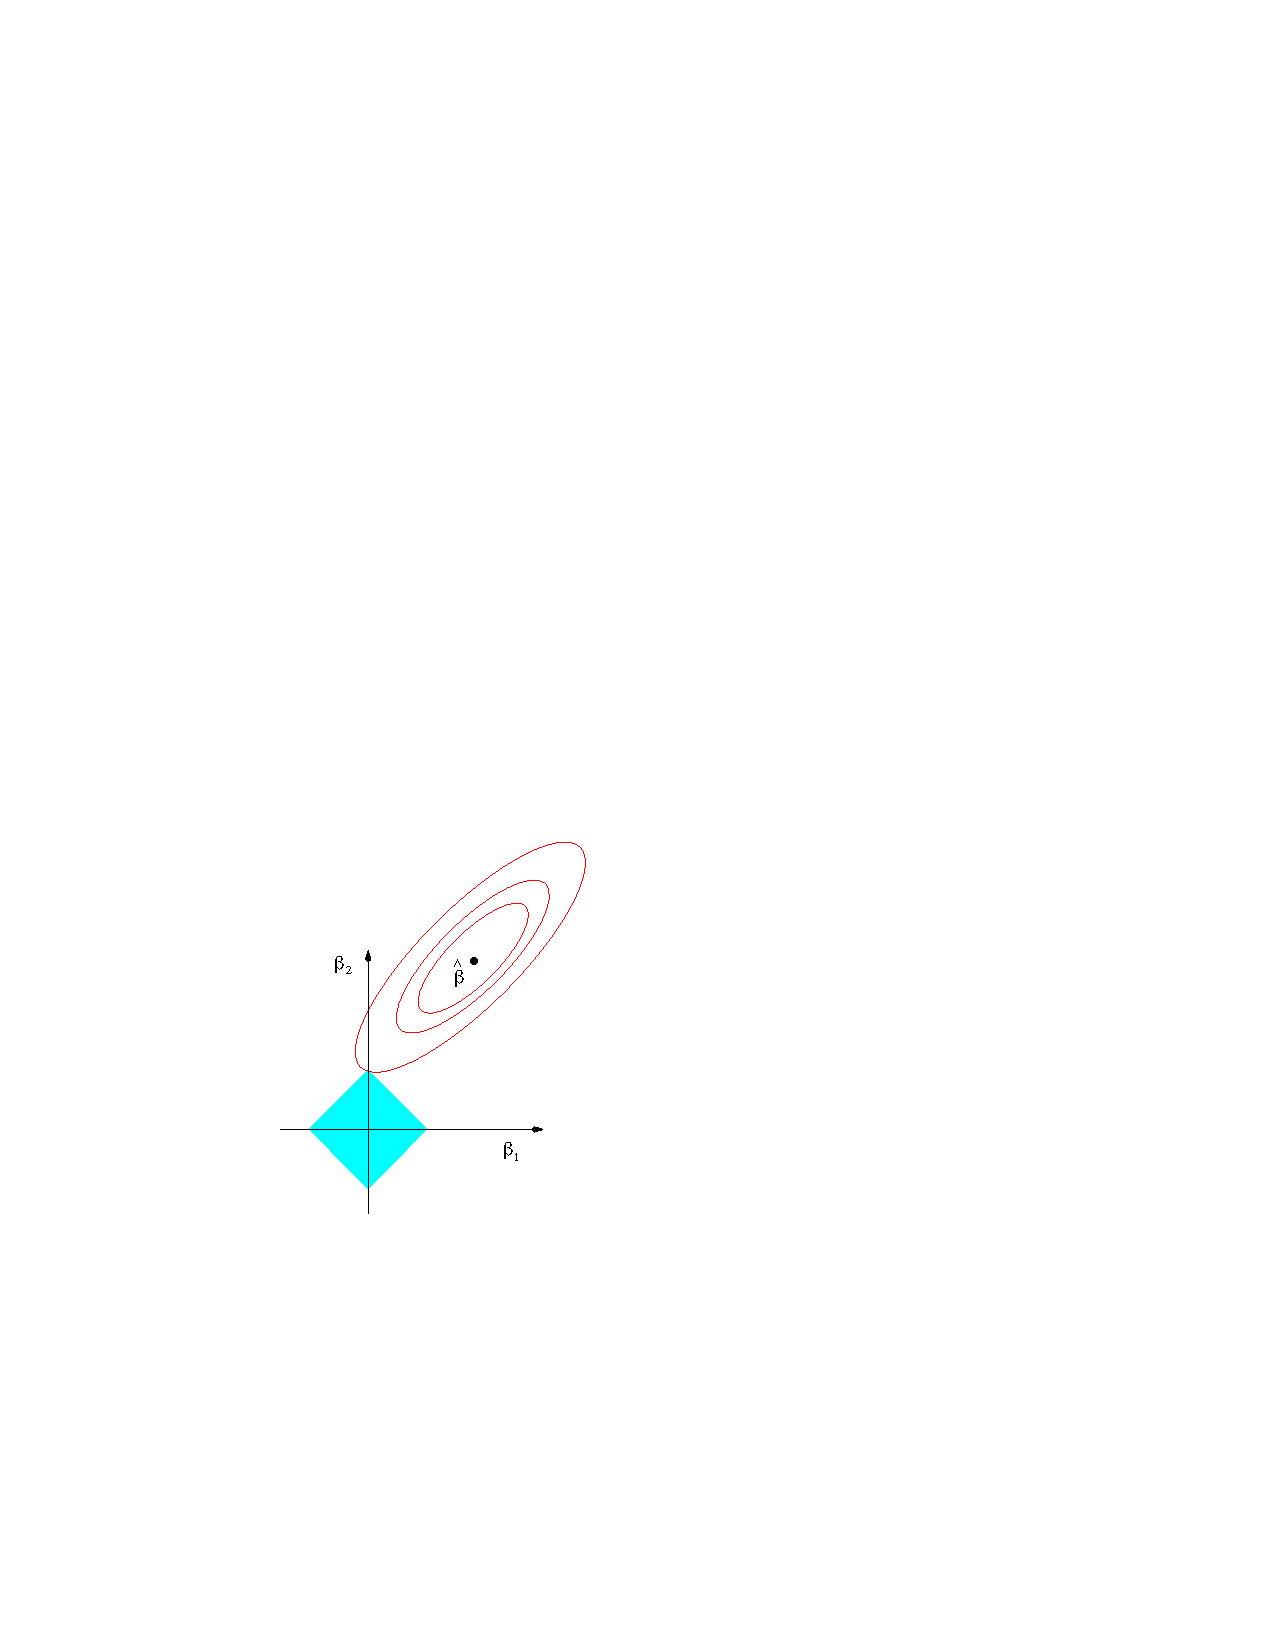
\includegraphics[scale=0.65]{RSE_lasso_constr}

\pause
\column{0.25\textwidth}
\begin{center}
Ridge.  Solutions must be in blue circle.
\end{center}
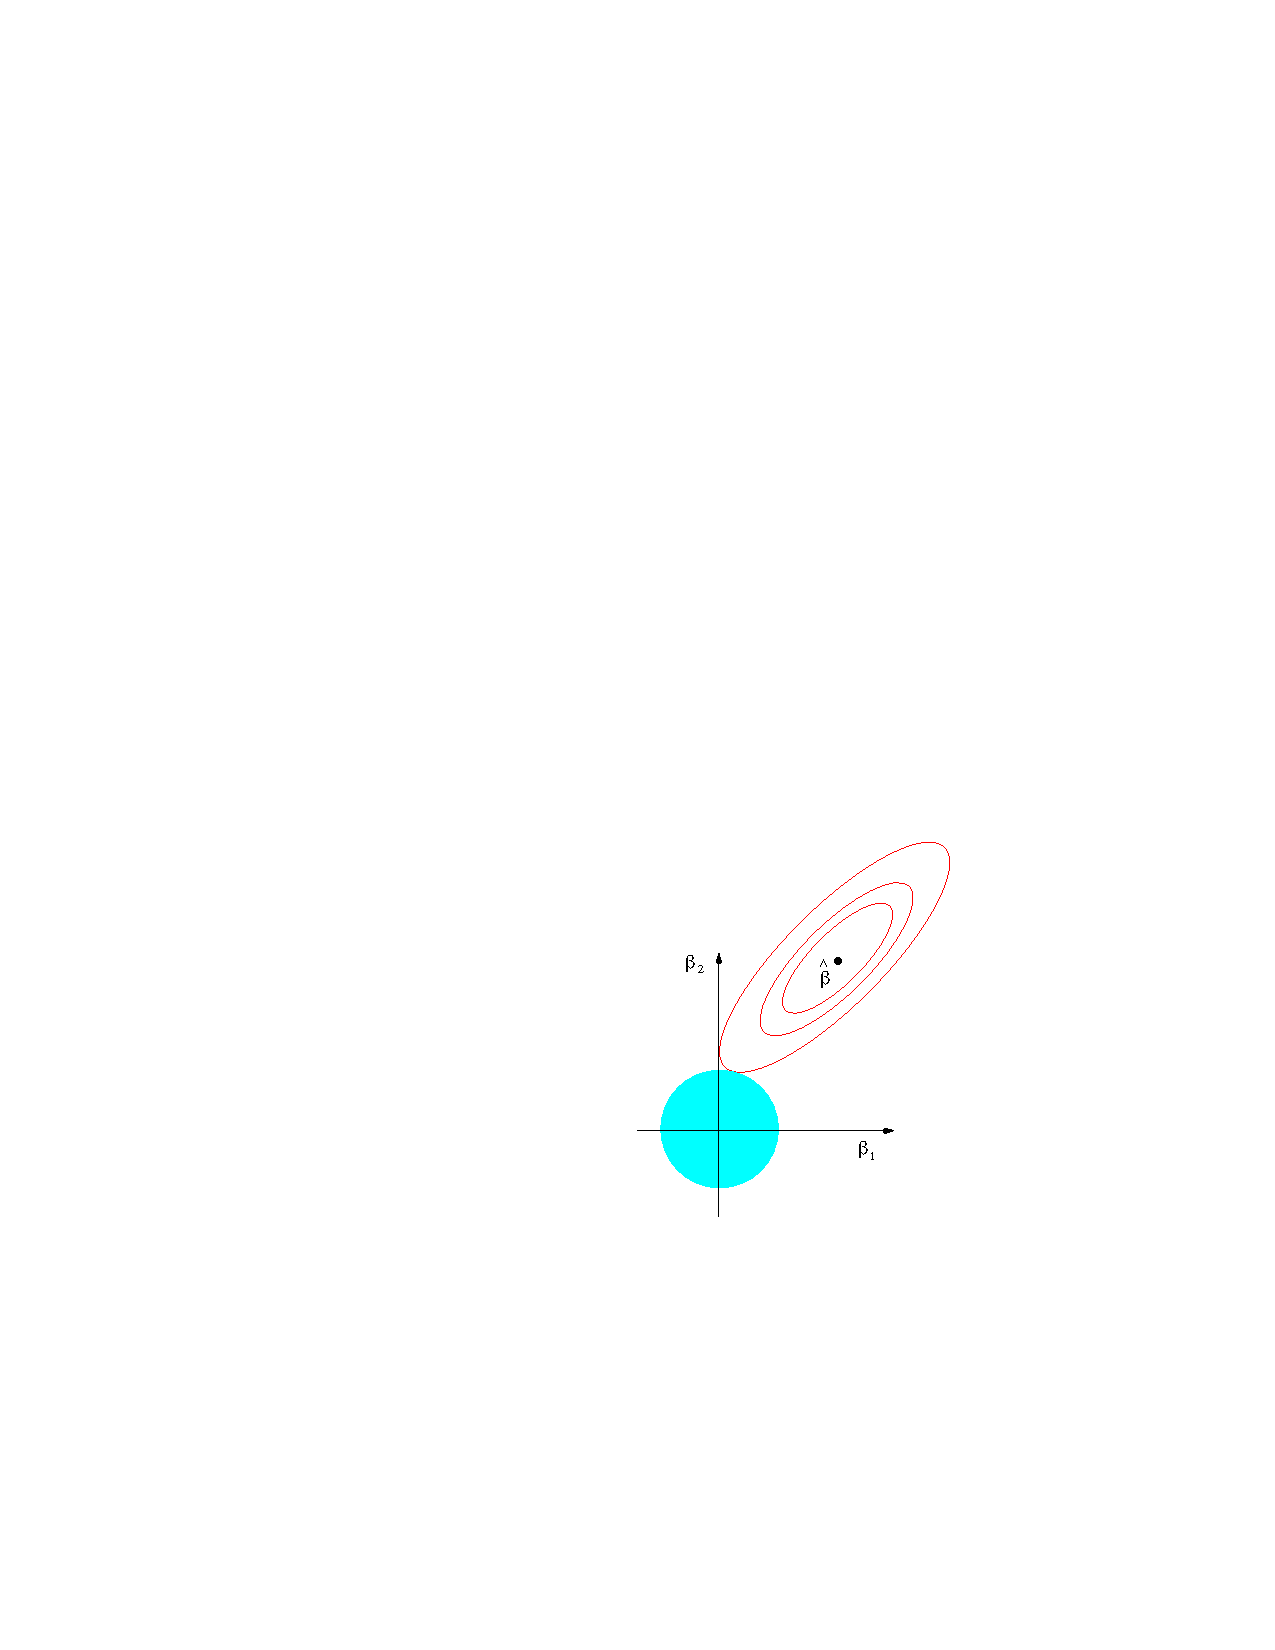
\includegraphics[scale=0.65]{RSE_ridge_constr}

\end{columns}

{\tiny Figures adapted from Elements of Statistical Learning}

\end{frame}

\begin{frame}{What do the parameter estimates look like?}
\begin{columns}
\column{0.6\textwidth}
\begin{figure}
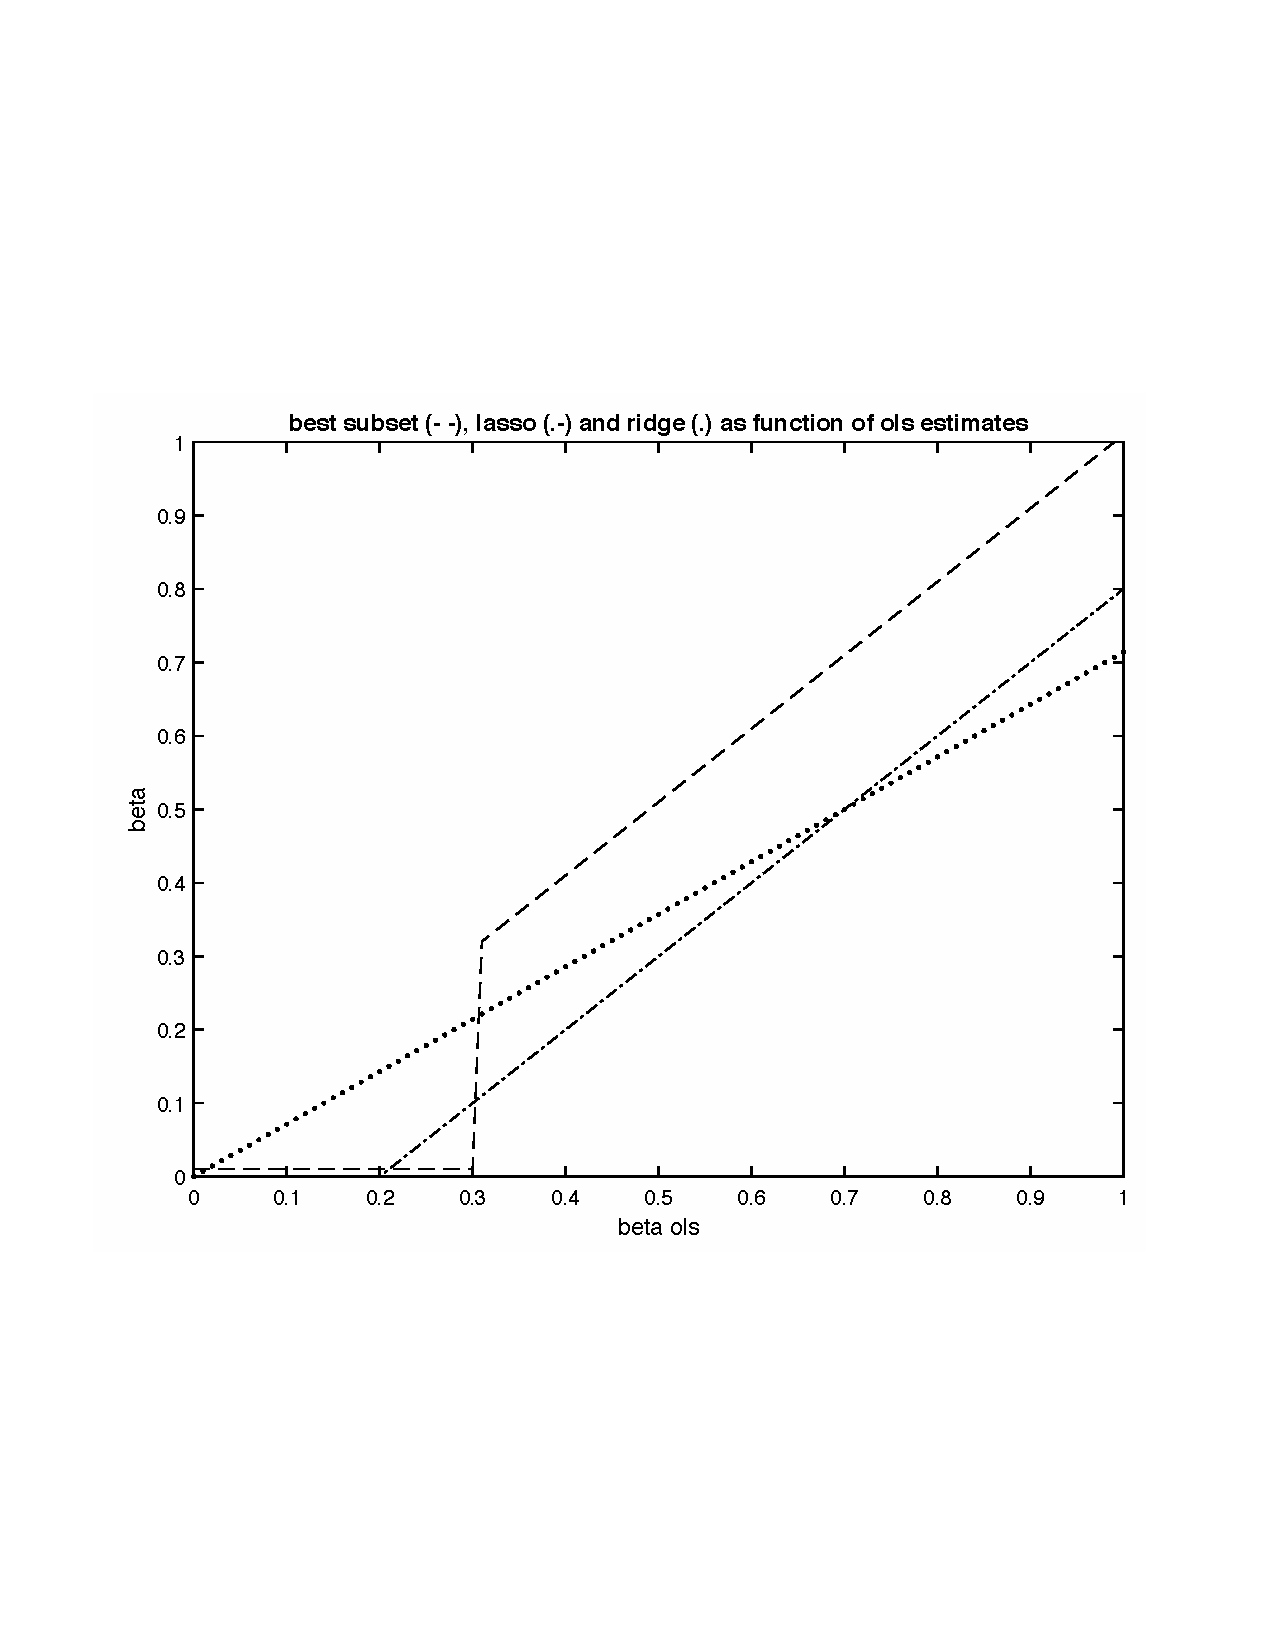
\includegraphics[scale=0.5]{lasso-ridge-subset-vs-ols}
\caption*{\tiny Figure taken from Imbens 2015 NBER lecture}
\end{figure}
\column{0.4\textwidth}
We often call regularization approaches ``shrinkage'' methods because, in general, they smoosh parameters closer to zero.
\end{columns}

\end{frame}


\begin{frame}{Objective 3}
Learn how the bias-variance tradeoff gets tuned with regularization term parameters. 
\end{frame}

\begin{frame}{Lasso or ridge?}


\begin{columns}
\column{0.5\textwidth}
Simulated data set from $n=50$ and $p=45$.  The response is a function of all 45 predictors.  Figure shows test MSE on y-axis.\\~\\
\begin{figure}
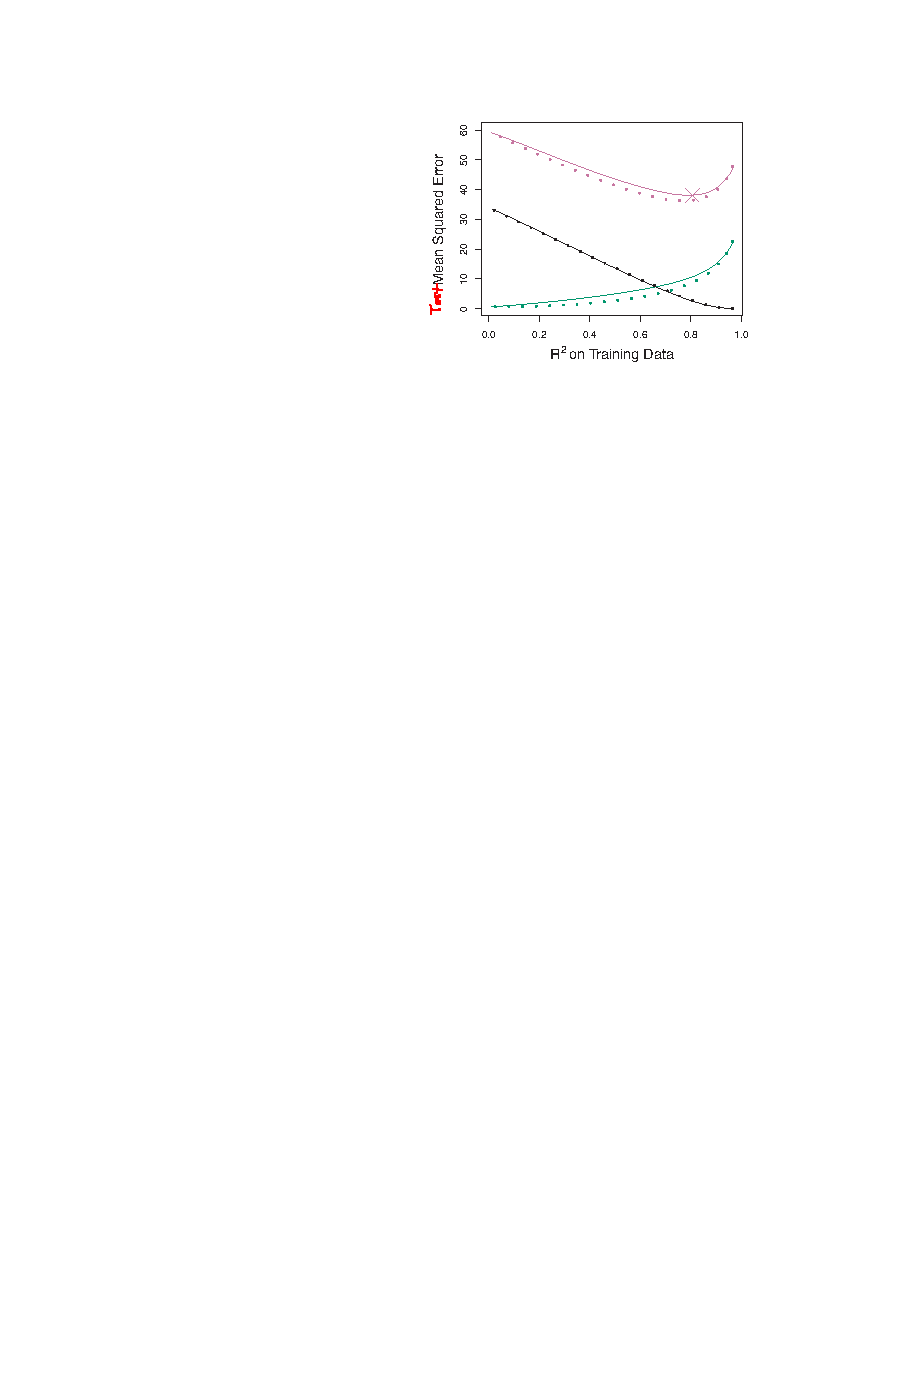
\includegraphics[scale=1]{lasso-v-ridge-45variables}
\end{figure}

\column{0.5\textwidth}
\uncover<2->{Simulated data set from $n=50$ and $p=45$.  The response is a function of only 2 of the 45 predictors.  Figure shows test MSE on y-axis.\\~\\
\begin{figure}
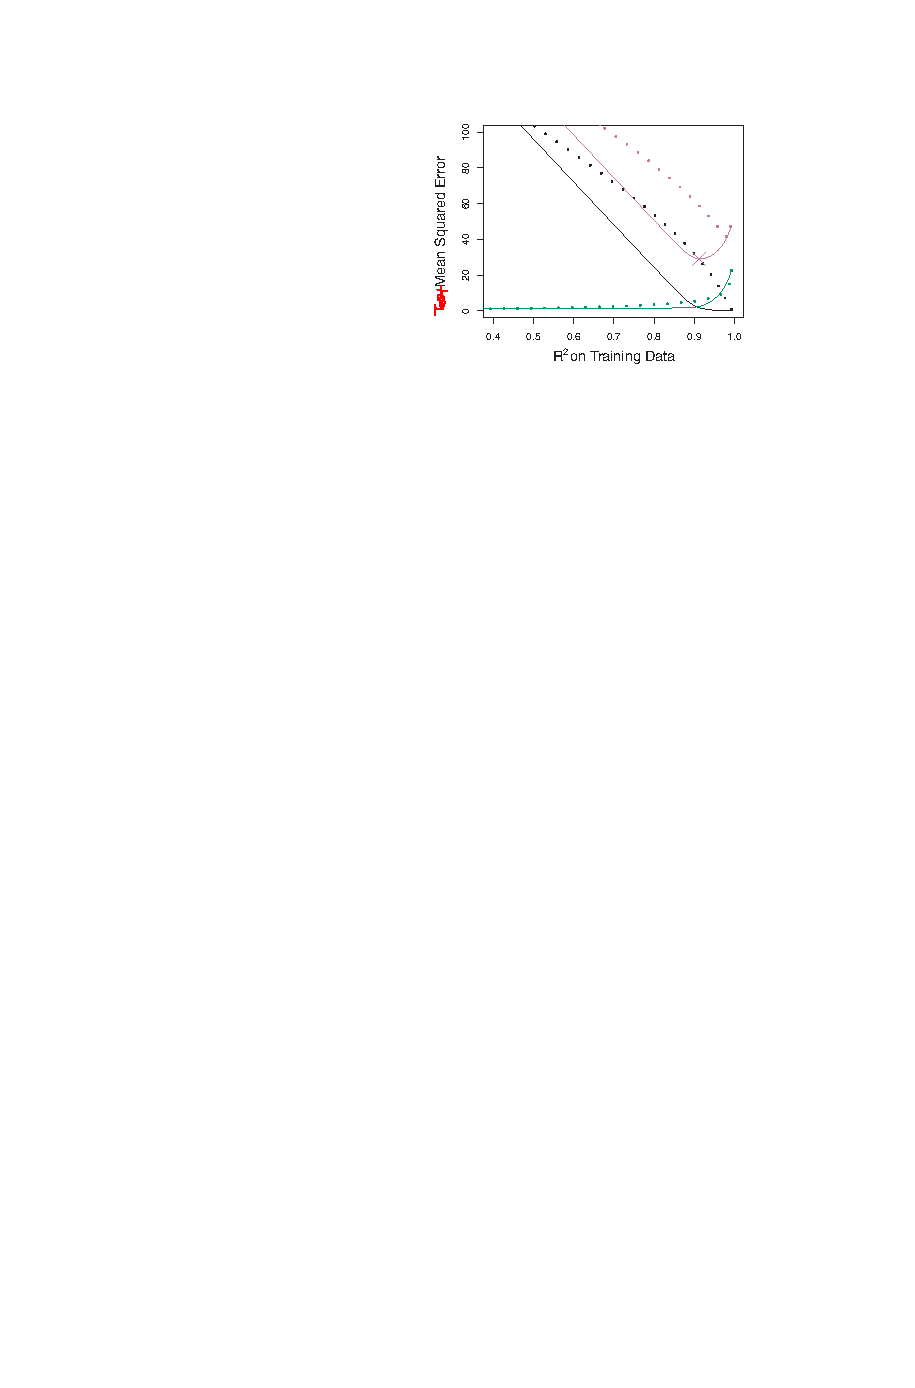
\includegraphics[scale=1]{lasso-v-ridge-2variables}
\end{figure}}

\end{columns}

Red show total MSE.  (Black and green are variance and bias.) 

Dashed line -- best Ridge.  Solid line -- best lasso.  
\end{frame}

\begin{frame}{Choosing $\lambda$}

As we've seen, $\lambda$ can take a range of values.  Here we see the tradeoff for the 2-of-45 predictors example  lasso example from the last slide. 


\begin{figure}
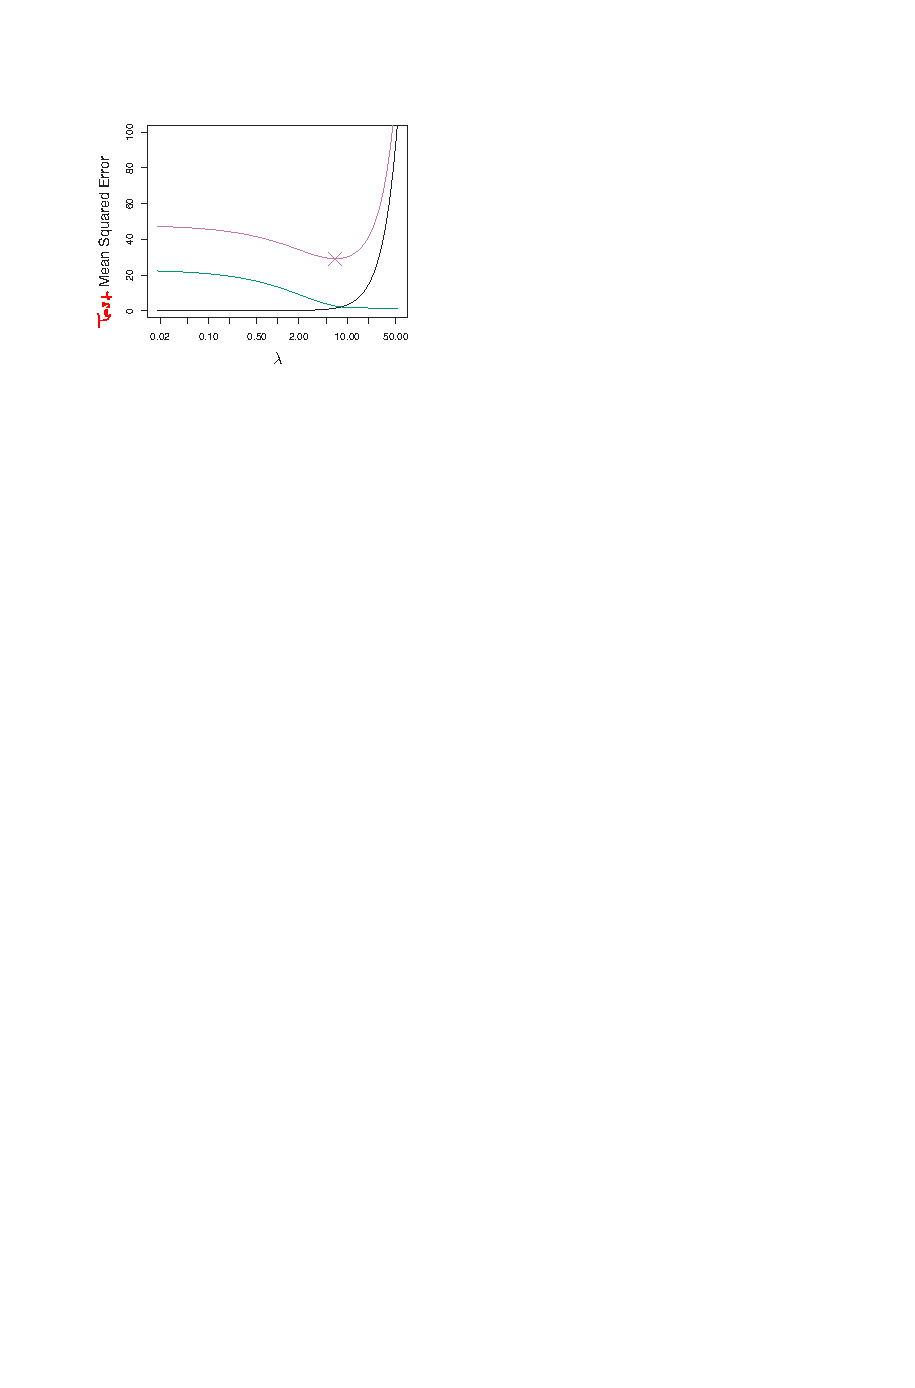
\includegraphics[scale=.85]{bias-variance-lasso-2}
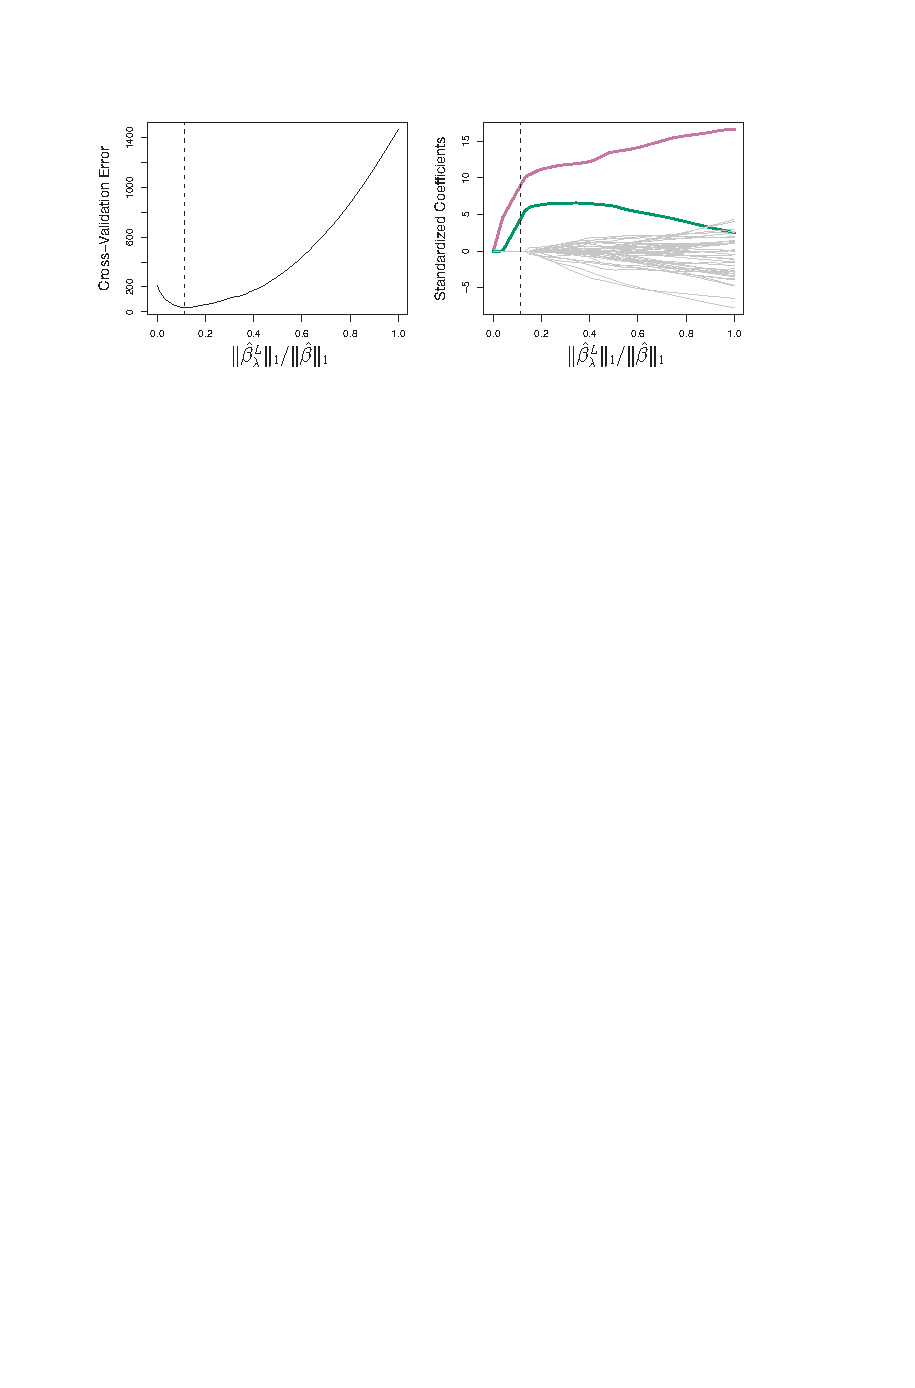
\includegraphics[scale=.85]{lasso-tenfold}
\end{figure}

\pause

Simple $\lambda$ selection strategy: use k-fold cross validation to test performance on a grid of $\lambda$ values. 


\end{frame}

\begin{frame}{Objective 4}

Understand the tradeoffs between these methods in more detail

\end{frame}

\begin{frame}{Lasso or ridge?}

Lasso performs better when the number of predictors truly is small, and otherwise it performs worse.  \\~\\

Since you can't know ahead of time if the response is a function of a few or all predictors, it makes sense to just try both.  

\end{frame}




\begin{frame}{Ridge regression advantages over OLS}

\pause

\textbf{First}.  Suppose some of your features are linear combinations of the others.  That means you can write $x_{i,j} = Ax_{i,-j}$ for at least 1 value of $j$. \\~\\

Then $\mathbf{X}^T\mathbf{X}$ is not ``full rank'' and you can't invert it.  I.e., $(\mathbf{X}^T\mathbf{X})^{-1}$ doesn't exist.

\begin{align*}
\text{e.g., }\mathbf{X}^T\mathbf{X} = 
\begin{bmatrix}
1 & 2 & 3\\
2 & 4 & 6\\
3 & 6 & 9
\end{bmatrix}
\uncover<3->{\text{ \quad vs.  \quad}
\mathbf{X}^T\mathbf{X} + \lambda \mathbf{I} =
\begin{bmatrix}
1+\lambda & 2 & 3\\
2 & 4+\lambda & 6\\
3 & 6 & 9+\lambda
\end{bmatrix} }
\end{align*}

\pause

But you \textit{can} invert $\left(\mathbf{X}^T\mathbf{X} + \lambda\mathbf{I}_k\right)$.  (Since you've added a little shift to the diagonals of the matrix, which restores linear independence)\\~\\



\pause

\textbf{Second.}  Computation!  It's faster than subset selection (but solves a different problem if your objective is parameter interpretation).

\end{frame}

\begin{frame}{Ridge regression advantages over OLS, ctd}

\textbf{Third.}  Bias-variance tradeoff! {\tiny Figure from ISLR}

\begin{columns}
\column{0.7\textwidth}
\begin{figure}
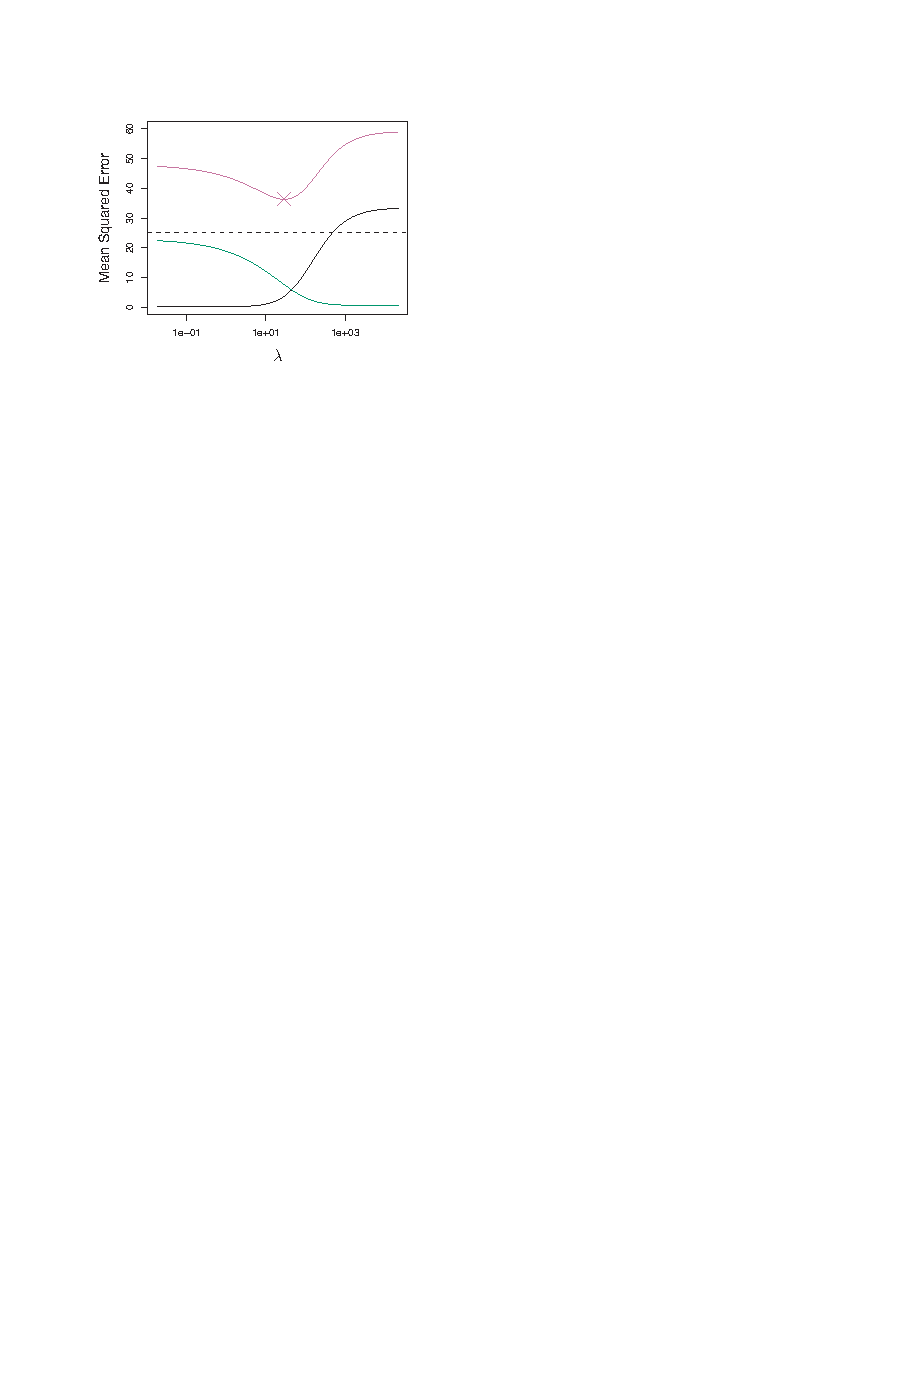
\includegraphics[scale=1.1]{bias-variance-ridge}
\end{figure}

\column{0.3\textwidth}

green: variance\\~\\
black: bias\\~\\
red: total error

\end{columns}

...but how can we choose $\lambda$?  The short answer is k-fold cross validation.

\end{frame}

\begin{frame}{Model selection tradeoffs}
\begin{table}[]
\begin{tabular}{p{6cm}p{2.2cm}p{2.2cm}p{2.2cm}}
\hline
                                              & Subset selection & Ridge    & Lasso \\ \hline
Computing time             \pause                   & high             & very low & low   \\
Drives parameters to zero?      \pause              & yes              & no       & yes   \\
Parameters biased relative to ``true'' model? \pause & no               & yes      & yes   \\
Easy to tune bias-variance?          \pause         & no               & yes      & yes   \\
Handles correlated features well?     \pause        & yes              & yes      & no    \\
Interpretability?	  \pause    & size of parameters & not really  & presence of parameters\\
 \hline
\end{tabular}
\end{table}

Lasso and ridge: 
\begin{itemize}
\item[$+$] less prediction variance than OLS, especially with many  predictors 
\item[$-$] more prediction bias than OLS
\end{itemize}
With highly correlated predictors, Lasso is unstable: indifferent between 
\begin{itemize}
\item $\hat{\beta}_1=0$ and $\hat{\beta}_2= \beta_1+\beta_2$
\item $\hat{\beta}_1= \beta_1+\beta_2$ and $\hat{\beta}_2=0$
\end{itemize}
\end{frame}

\begin{frame}{Objective 5}

Normalize your variables!

\end{frame}

\begin{frame}{Normalizing variables}

For ridge and lasso, it's important to ``normalize" your variables:

\begin{equation}
x' = \frac{x - \bar{x}}{\sigma_x}
\end{equation}

...and then fit the model to the normalized values.  \\~\\

Any guesses why?\\~\\

\pause

Reason: This way variables with large numeric values don't dominate the solution.  

\end{frame}

\begin{frame}{Hot topic:  Elastic nets...}

\begin{columns}
\column{0.5\textwidth}
...are cool!\\~\\

Elastic nets
\begin{itemize}
\item Drive parameters to zero like lasso
\item Deals with correlated predictors well, like ridge (by shinking them together)
\item Give you another !\&@!\%* parameter to tune
\item Still aren't always best -- good to try several shrinkage methods, not just this.
\end{itemize}

\column{0.5\textwidth}

\begin{align*}
\lambda \sum_{k=1}^K  \left(\alpha \beta_j^2 + (1-\alpha) |\beta_j|\right)
\end{align*}


\begin{figure}
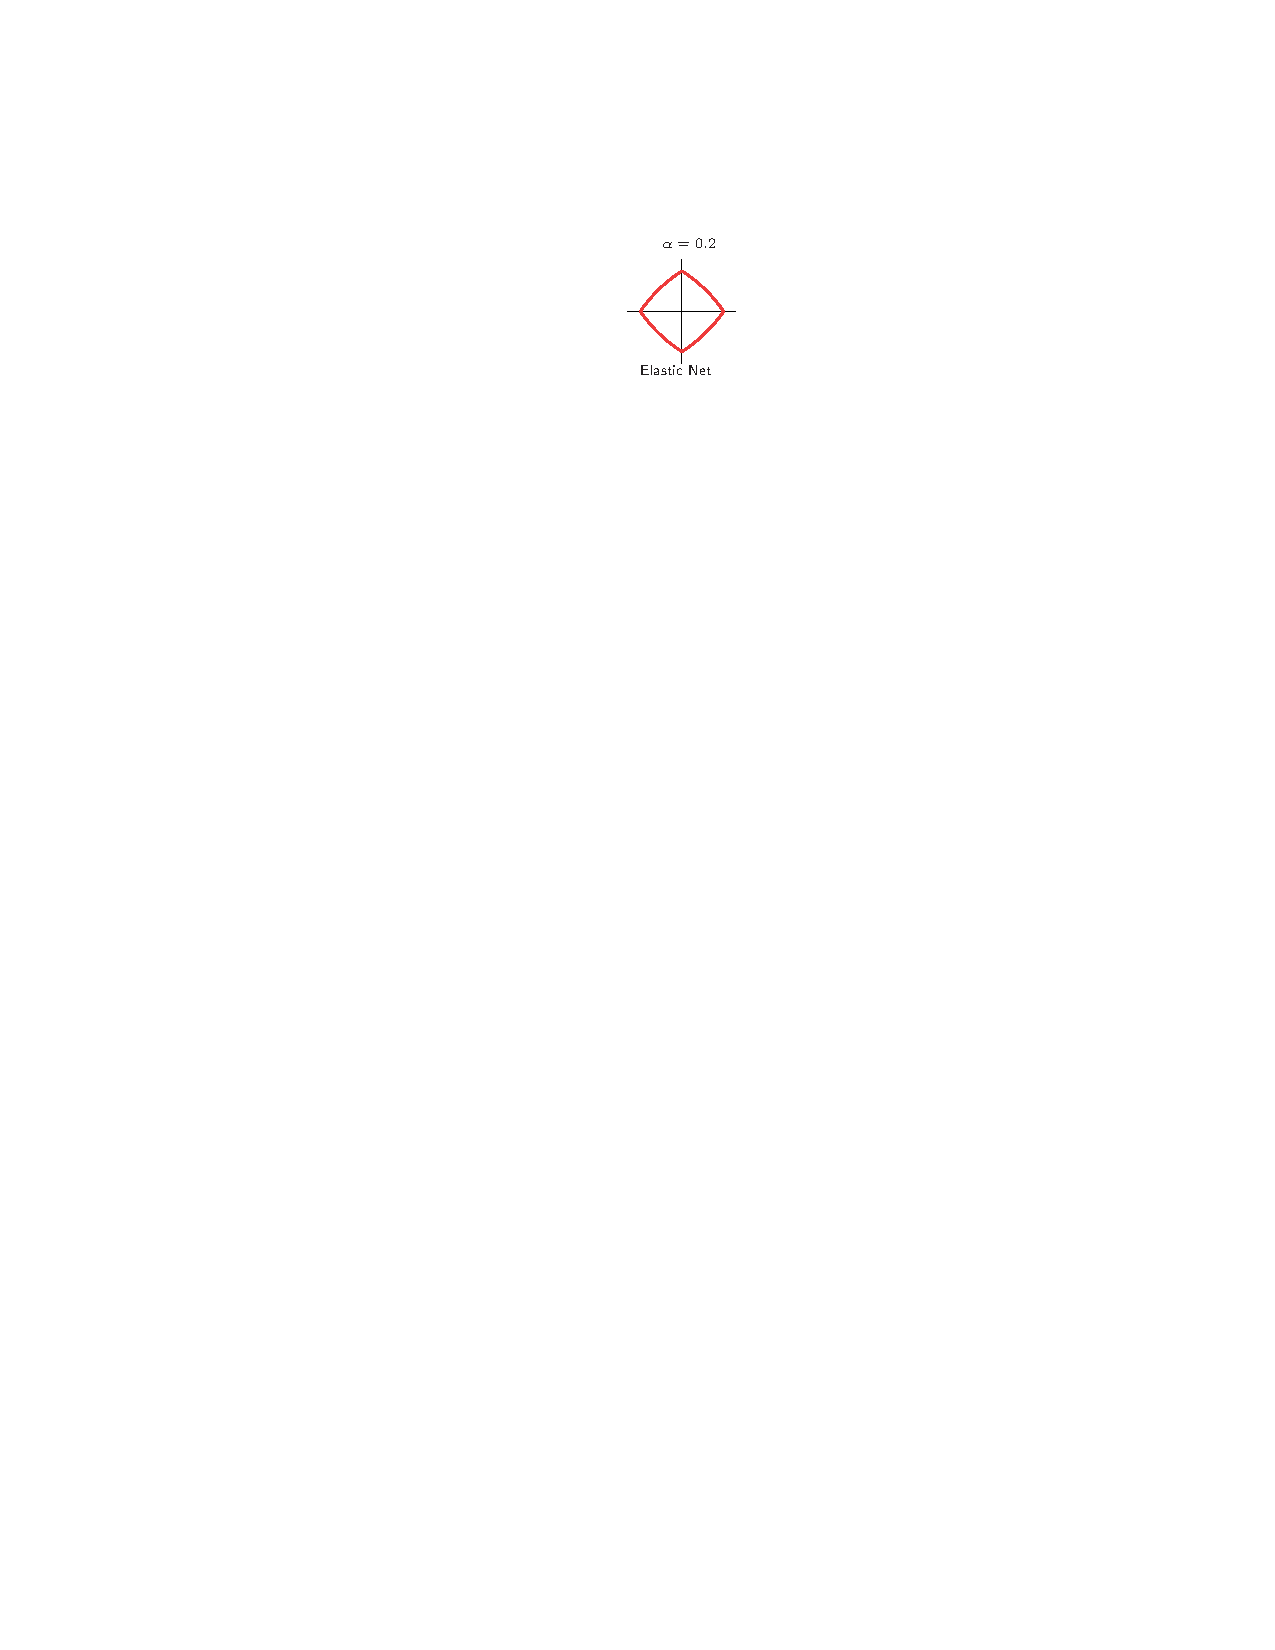
\includegraphics[scale=1]{elastic-net}
\caption*{\tiny from Elements of Statistical Learning}
\end{figure}

\end{columns}
\end{frame}

\begin{frame}{Reading questions}

\begin{itemize}
\item What are their main answers to the question posed in Section 1.2, "Why Find Spatial Predictions for Ozone?"
\item Section 2.1: Why do the authors average their data?  Could they be missing anything important by doing this?
\item Section 4.1: Be prepared to describe in words the model the authors are fitting to the data.  Is this a meaningful model to estimate?  Why or why not?
\item Section 4.2, paragraph 3 to end of Section 4.2:  How does their formulation of the lasso procedure differ from what we learned in class?  Can you see how the two formulations could get similar results?  How does $\lambda$ in the formulation we learned relate to $t$ in the formulation presented in this paper? 
\item Section 4.3: Be prepared to comment on their model validation procedure.  How might you improve on it?  What problems are they exposed to by taking the approach they do?
\item Interpretation.  Think about ways in which this approach might be practically applied to improving our understanding of air quality.  Can it be adapted to address equity issues in situations where monitoring stations are sparse?
\end{itemize}
\end{frame}

\end{document}
